\documentclass[10pt,twocolumn,letterpaper]{article}

\usepackage{cvpr}
\usepackage{times}
\usepackage{epsfig}
\usepackage{graphicx}
\usepackage{amsmath}
\usepackage{amssymb}
\usepackage{graphicx}

% ------ New Package Here ------

\usepackage{caption}
\usepackage{dblfloatfix}
\usepackage{subcaption}
\usepackage{bm}
\usepackage[pagebackref=true,breaklinks=true,letterpaper=true,colorlinks=true,bookmarks=true]{hyperref}
% ------------------------------

\makeatletter
\newcommand\footnoteref[1]{\protected@xdef\@thefnmark{\ref{#1}}\@footnotemark}
\makeatother
% --------Settings-------------------------------------
\setlength{\belowcaptionskip}{-5pt}
\setlength{\abovecaptionskip}{0pt}
%---------MATH SYMBOLS NEW COMMANDS:--------------------------------------
\newcommand{\vectornorm}{|}

\newcommand{\diver}{\mathrm{div}}
\newcommand{\grad}{\mathrm{grad}}
\newcommand{\trace}{\mathrm{trace}}
\newcommand{\ud}{\mathrm{d}}

\newcommand{\mvec}[1]{\boldsymbol{#1}}
\newcommand{\matr}[1]{\mathrm{#1}}

\newcommand{\eye}{\mathrm{I}}
\newcommand{\img}{u}

\newcommand{\prob}[1]{\mathrm{p}\left( #1 \right)}

\newcommand{\bhat}{\widehat{\mvec{b}}}
\newcommand{\lamhat}{\widehat{\mvec{\lambda}}}
\newcommand{\eps}{\mvec{\varepsilon}}

%\newcommand{\norm}[1]{\left\Vert#1\right\Vert}
% \newcommand{\norm}[1]{\left \|#1 \right \|}
\newcommand{\norm}[1]{\left |#1 \right |}
\newcommand{\transp}{^\mathrm{T}}

\newcommand{\bu}{\boldsymbol{u}}
\newcommand{\bx}{\boldsymbol{x}}
\newcommand{\bp}{\boldsymbol{p}}

\newcommand{\be}{\boldsymbol{\varepsilon}}

\newcommand{\bv}{\boldsymbol{v}}
\newcommand{\mfsf}[0]{{\sc mfsf}}
\newcommand{\mfsfc}[0]{{\sc mfsf\em c}}
\newcommand{\mfsfdct}[0]{{\sc mfsf$_{\tt DCT}$}}
\newcommand{\mfsfpca}[0]{{\sc mfsf$_{\tt PCA}$}}
\newcommand{\mfsfid}[0]{{\sc mfsf$_{\tt I_{2F}}$}}
\newcommand{\mfsfcdct}[0]{{\sc mfsf\em c$_{\tt DCT}$}}
\newcommand{\mfsfcpca}[0]{{\sc mfsf\em c$_{\tt PCA}$}}
\newcommand{\mfsfcid}[0]{{\sc mfsf\em c$_{\tt I_{2F}}$}}


\newcommand{\cU}{\mathcal{U}}
\newcommand{\bU}{\boldsymbol{\mathcal{U}}}
\newcommand{\bE}{\boldsymbol{\mathcal{E}}}
\newcommand{\bI}{\boldsymbol{I}}
\newcommand{\bA}{\boldsymbol{A}}
\newcommand{\bb}{\boldsymbol{b}}
\DeclareMathOperator*{\argmin}{arg\,min}
\DeclareMathOperator*{\argmax}{arg\,max}


\newcommand{\bL}{\boldsymbol{L}}
\newcommand{\bM}{\boldsymbol{M}}

\newcommand{\R}{\mathbb{R}}

\newcommand{\Lone}{\mathbf{L}^1}
\newcommand{\Ltwo}{\mathbf{L}^2}


%----------------------------------------------------------------------------------------------------


% \iccvfinalcopy % *** Uncomment this line for the final submission

\def\cvprPaperID{0008} % *** Enter the cvpr Paper ID here
\def\httilde{\mbox{\tt\raisebox{-.5ex}{\symbol{126}}}}

% Pages are numbered in submission mode, and unnumbered in camera-ready
\ifcvprfinal\pagestyle{empty}\fi

\begin{document}

%%%%%%%%% TITLE
\title{Supplementary Material \\ Estimating Correspondences of Deformable Objects ``In-the-wild"}
\author{Yuxiang Zhou$^\star$ \hspace{0.5cm} Epameinondas Antonakos$^\star$ \hspace{0.5cm} Joan Alabort-i-Medina$^\star$ \hspace{0.5cm} Anastasios Roussos$^\star$ \\ Stefanos Zafeiriou$^{\star, \dagger}$\\
$^\star$Department of Computing, Imperial College London, U.K.\\
$^\dagger$Center for Machine Vision and Signal Analysis, University of Oulu, Finland\\
{\tt\small \{yuxiang.zhou10, e.antonakos, ja310, troussos, s.zafeiriou\}@imperial.ac.uk}}

\maketitle
\thispagestyle{empty}


%%%%%%%%% Appendix
\section*{Introduction}
In this supplementary material, we provide additional experimental results and comparisons for the proposed pipeline of constructing both Dense AAMs and Patch-based AAMs. 
For \textbf{Dense AAM}, We present more detailed algorithms explanation and intrinsic property analysis of Dense AAMs. In section~\ref{sec:cost_function},  minimisation of the energy function are described in more details. In Section \ref{sec:daam_fittingresults}, we present visualisations of in-the-wild model fitting  for faces and ears, comparing classic AAMs and the proposed dense AAMs. In Section \ref{sec:modelanalysis}, we provide evaluations and comparisons of dAAMs, in terms of model compactness, warping quality and reconstruction accuracy. 
For \textbf{Patch-based AAM}, we described how sparse landmark points are sparsely sampled from dense reference shape and mapped to rest shapes according to dense correspondences in section~\ref{sec:sparsesample}. A visualisation for Patch-based AAM shape model is presented in section~\ref{sec:paam_sm}. Also more visualisation of fitting results are shown in section~\ref{sec:paam_fittingresults}.















\appendix
\section{Dense Active Appearance Model}
\label{sec:daam}
This section presents 1) detailed description of minimising cost function, 2) intrinsic property analysis of dense AAM and 3) visualisation of fitting dense AAMs on faces and ears.

\subsection{Detailed Cost Function Description}
\label{sec:cost_function}

\begin{figure}[!t]
\centering
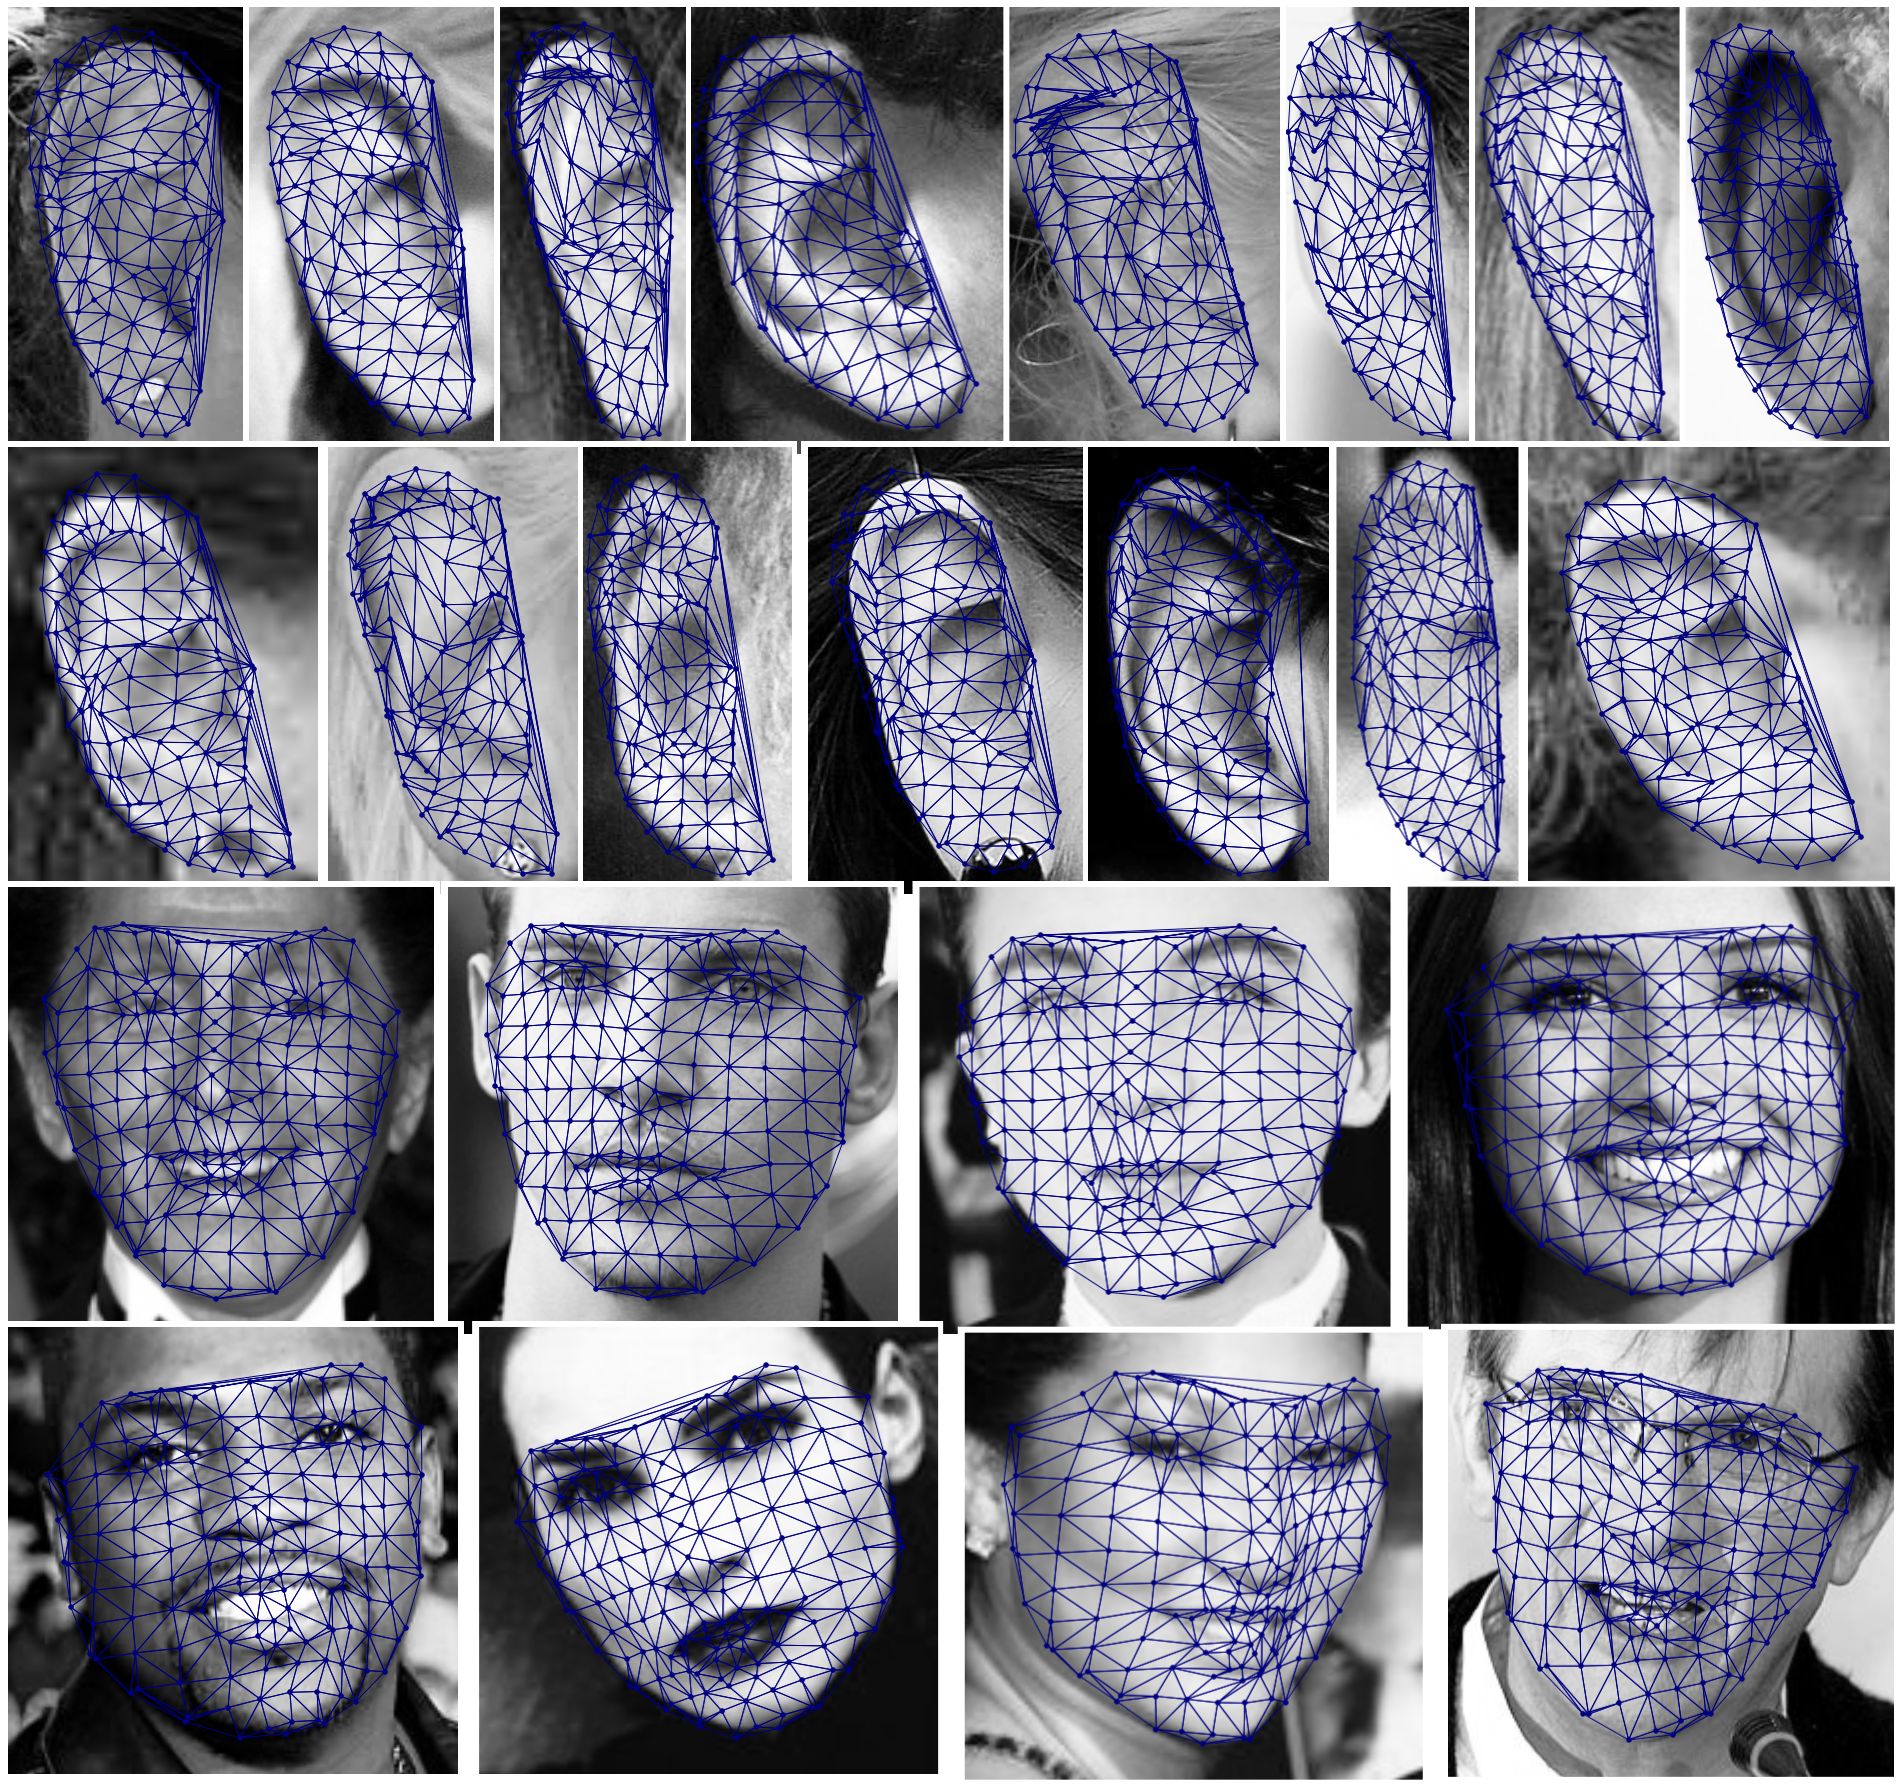
\includegraphics[width=0.5\textwidth]{Suplementory_Meterial/Fittings/fittings}
\caption{Result of fitting dAAMs on ears (first two rows) and faces (last two rows). A dense grid visualisation is used.}
\label{fig:fr}
\end{figure}

\begin{figure*}[!t]
\centering
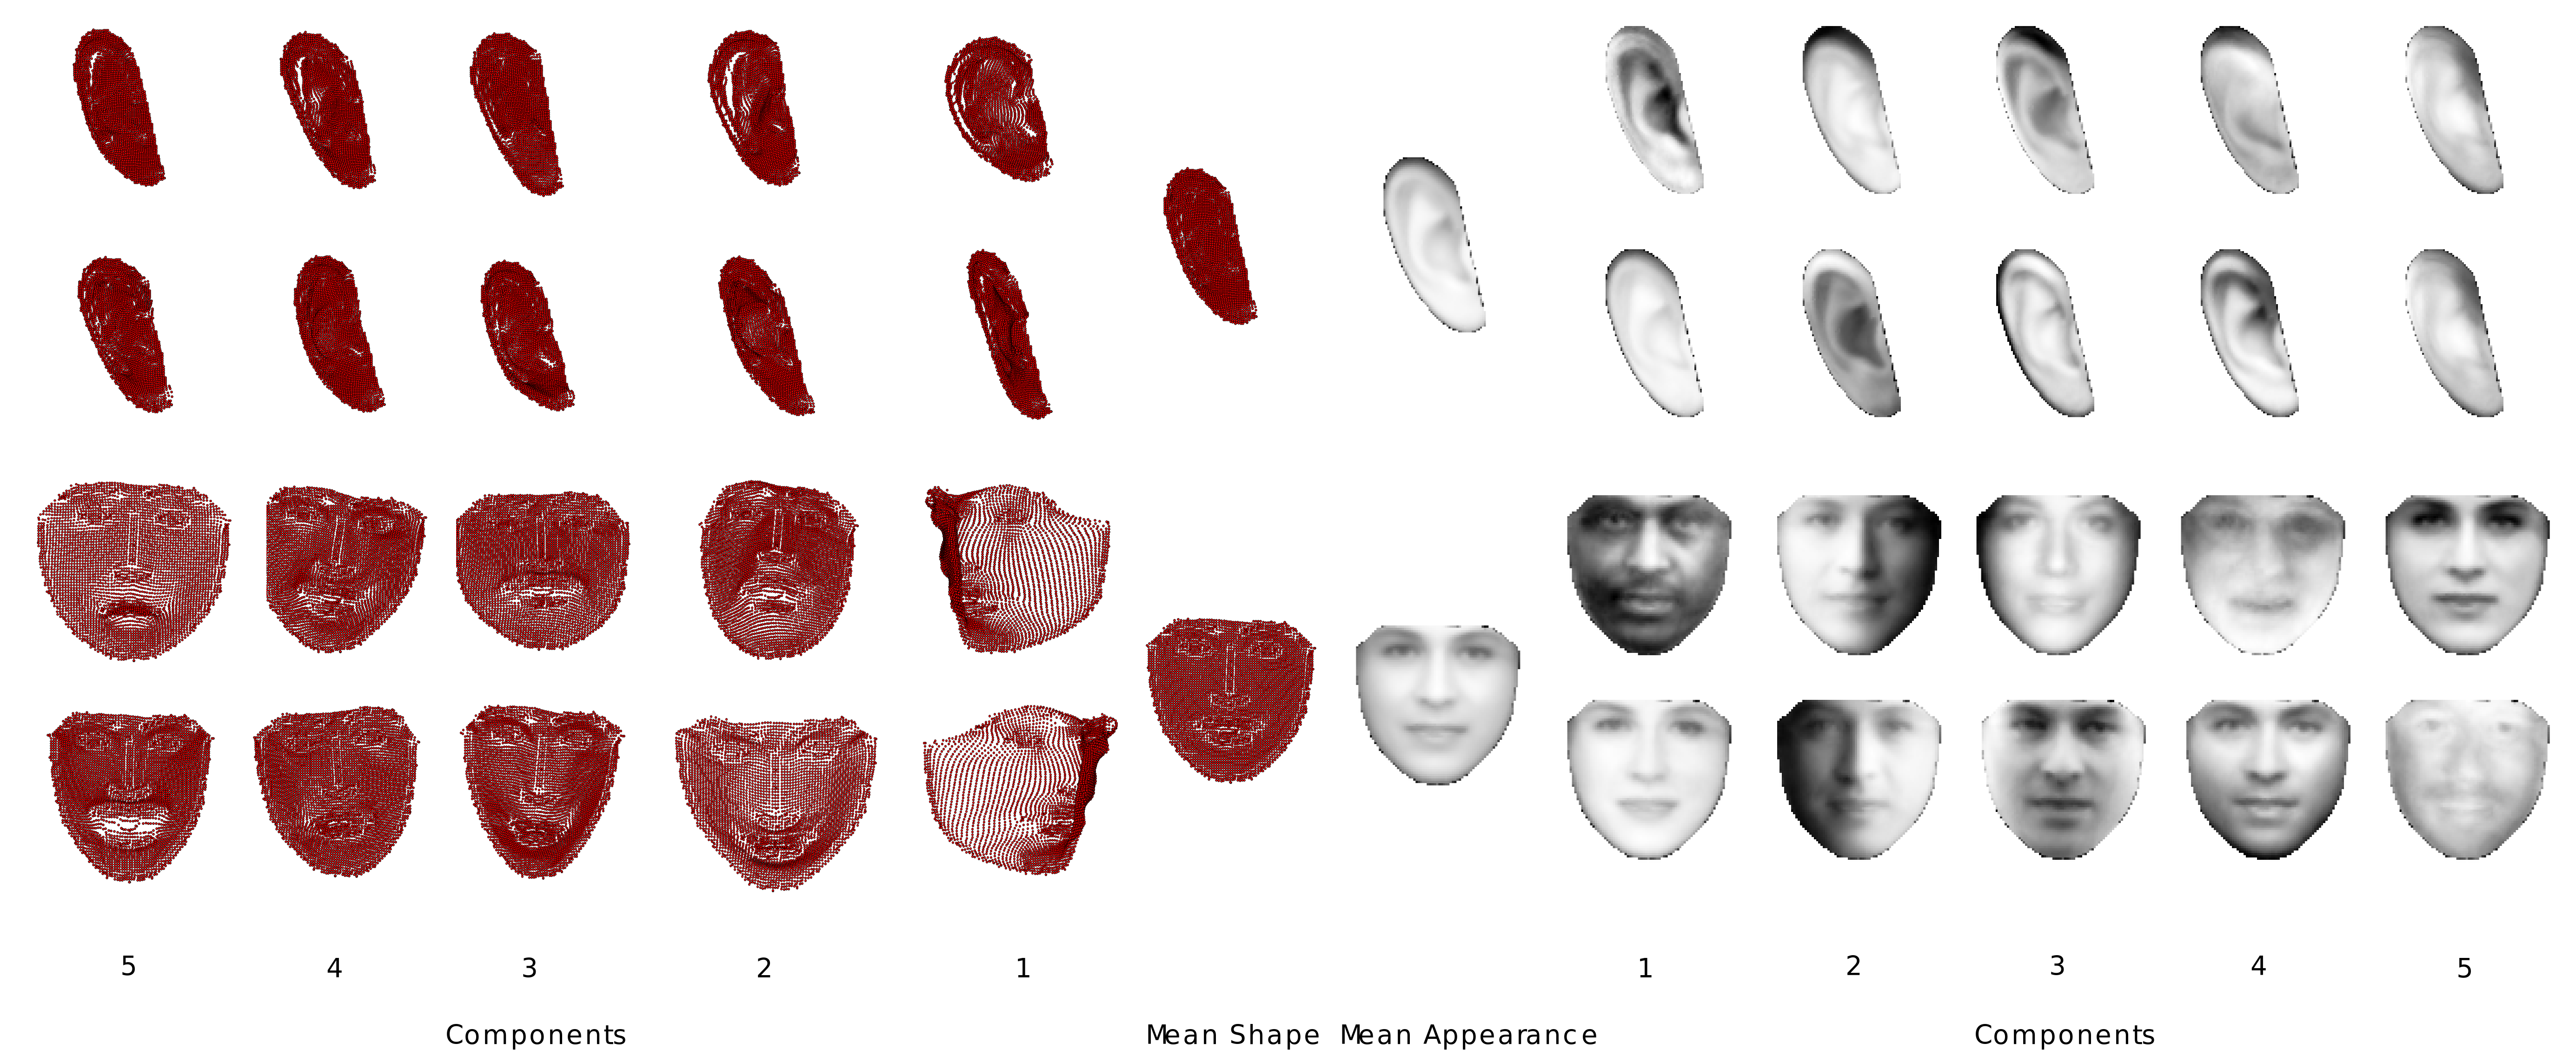
\includegraphics[width=\textwidth]{Suplementory_Meterial/Models/models}
\caption{Principal components of dAAMs built on ears (top) and faces (bottom). The mean (middle columns) as well as the first five principal components are visualised for both shape (left) and appearance (right). $\pm 3$ times the variance of the corresponding component is used in each case.}
\label{fig:pcamodel}
\end{figure*}

Using the SVS functions built from training data, one of the main steps of our pipeline is to estimate dense correspondences between all these functions. We propose to perform this estimation simultaneously for all training data, by using the correspondence basis.

In order to learn the such a subspace, we first transform the original annotation to point clouds. Then, we use NICP to align the previous point clouds with respect to a reference point cloud template. NICP iteratively deforms each point cloud until its points match the ones on the shape template and correspondences are established. However, because optical flow is a pixel-wise frame registration technique, we need to establish correspondences for all pixels on the reference frame rather than for sparse point clouds. To achieve this, we apply Thin Plate Spline (TPS) \cite{Bookstein1989} to find correspondences for all pixels in the reference frame given the point cloud correspondences provided by the previous NICP stage. Once dense correspondences have been established among all pixels, the so-called correspondence subspace is obtained by performing PCA the trajectory of all pixels. Note that incorporating the previous subspace as a low rank constrained in optical flow is consistent with its assumption of smooth motion.

In every coarse-to-fine and warping iteration, we use an initialization that comes from the previous iteration and for the very beginning, we initialize with a Thin Plate Splines (TPS) \cite{Bookstein1989} interpolation of the initial correspondence vectors described in Sec.~\ref{sec:step2}. We approximate the data term \eqref{eq:costfunc} by linearizing the SVS images around the initialization. After that, the energy becomes convex and we optimize it using alternating optimization w.r.t.~$\bm{v}_i(\bx)$ and $\bm{u}_n(\bx)$. The minimization w.r.t.~
$\bm{v}_i(\bx)$ is decoupled for every coefficient $i$ and corresponds to Rudin-Osher-Fatemi Total Variation denoising \cite{rudin92}, which we solve efficiently by applying the first order primal-dual algorithm of \cite{Chambolle:Pock:JMIV2011}. The minimization w.r.t.~
$\bm{u}_n(x)$ is decoupled for every pixel $\bx$ and every shape index $i$. This minimization is also implemented by applying the efficient primal-dual algorithm of \cite{Chambolle:Pock:JMIV2011}.

To register all decision functions to temp`late shape, decision function $d_i(\bm{x}), i \in {1,...,F}$ are grouped into one sequence before applying flow algorithm. The objective cost function we would like to minimise is:
\begin{align}
    \operatorname*{arg\,min}_{\bm{u}_n(\bm{x}), \bm{v}}&=\alpha \int_{\Omega}\sum_{n=1}^F|\bm{d_n}(x+\bm{u}_n(x))-\bm{d_0}(x)\| dx  \label{eq:costfunc}\\
    &+ \beta \int_{\Omega}\sum_{n=1}^F\|\bm{u}_n(x)-\sum_{i=1}^R\bm{q_i}(n)\bm{v_i}(x)\|^2 dx \label{eq:lowrank}\\
    &+ \sum[\bm{TV}(Qv)]
\end{align}
where $d_n(x)$ is the decision function from~\eqref{eq:decisionfunc}, which returns possibilities of given coordinate classified as shape component where coordinates are from set $\Omega \in \Re^2$. $TV(Qv)$ is total variation as regularization on low rank subspace, $Q$ is trajectory basis and $v^T.L.v$ is low rank spacial constrains.

Term~\eqref{eq:costfunc} state the shape constancy where points having similar classification probability are from same object.
Part~\eqref{eq:lowrank} applies constrain on low rank trajectory basis states in section~\ref{sec:trabasis}.
The objective cost function has two free parameters $u$ and $v$, so we perform alternating minimisation. The equation can be solved using a thresholding scheme after linearisation of image functions. The minimisation can be speed up by paralleling the minimisation for every spatial-temporal point $(x;n), x \in \Omega, n \in \{1,...F\}$ independently.

After solving the equation, $\bm{u}_n(\bm{x}), x \in \Omega$ gives a group of deformation fields that registering every decision functions in the shape sequence to reference frame e.g. $\bm{u_1}(\bm{x})$ registers decision function $\bm{d_1}(\bm{x})$ to the reference frame. Figure~\ref{fig:deformationfield} demonstrates deformation fields that warps from reference frame where there is no deformation.

Applying PCA on deformations trains dense deformable shape model:
\begin{equation*}
    \bm{s_p}=\bm{\bar{s}} + \bm{U}_s\bm{p}
\end{equation*}
where $\bm{s_p}$ is deformed shape instance. $\bm{\bar{s}}$ is mean shape and $\bm{U}_s\bm{p}$ are eigenvectors with corresponding parameters $p$. 


\subsection{Fitting Results}
\label{sec:daam_fittingresults}
This section provides additional visualisations for the experiments of Section 3.3 of the main submission (Non-rigid object alignment in-the-wild). We visualise pixel-wise dense fitting results for both faces and ears. Results for this experiment of faces are reported over the 224 testing images of the LFPW database using 68 point ground truth landmark annotations
\footnote{\label{ibug_300} \url{http://ibug.doc.ic.ac.uk/resources/300-W/}}.
For ears, we collected 605 high resolution images of ears in unconstrained scenarios and annotated them using both a newly defined 55 point annotation scheme for ears and the curve annotations proposed in the paper. Results for fitting ears are reported over 105 testing images.

Figure \ref{fig:fr} shows dense fitting results using a grid visualisation, thus dense points are visible without affecting the visibility of appearance.


\subsection{Shape Model Analysis}
\label{sec:modelanalysis}



\begin{figure}[!b]
    \centering
    % \vspace*{-0.1in}
    \begin{subfigure}[b]{0.43\textwidth}
            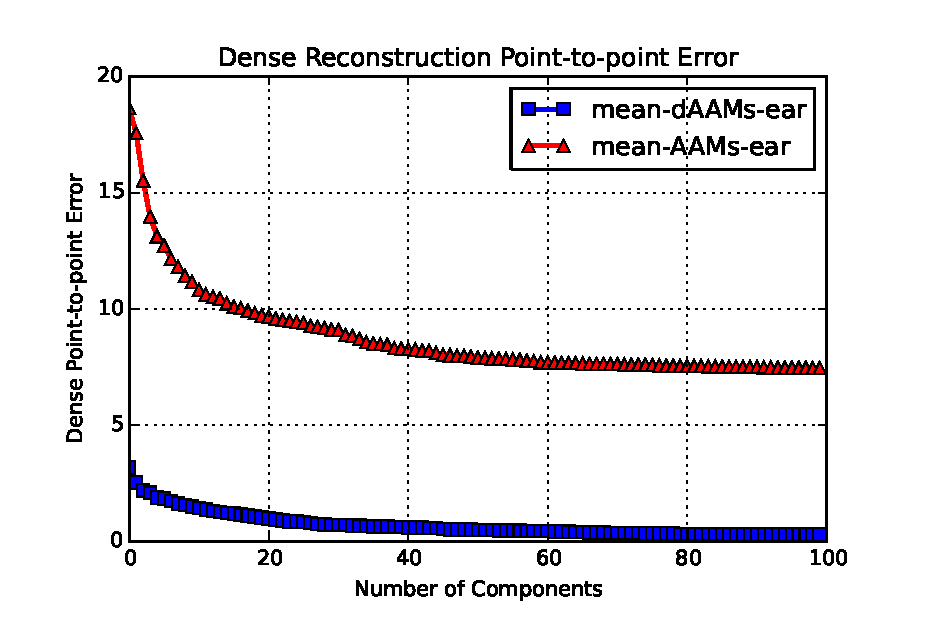
\includegraphics[width=\textwidth]{Suplementory_Meterial/Model_Analysis/sr_ear}
        %\caption{dAAMs dense shape reconstruction}
    \end{subfigure}
    \\
    \begin{subfigure}[b]{0.43\textwidth}
            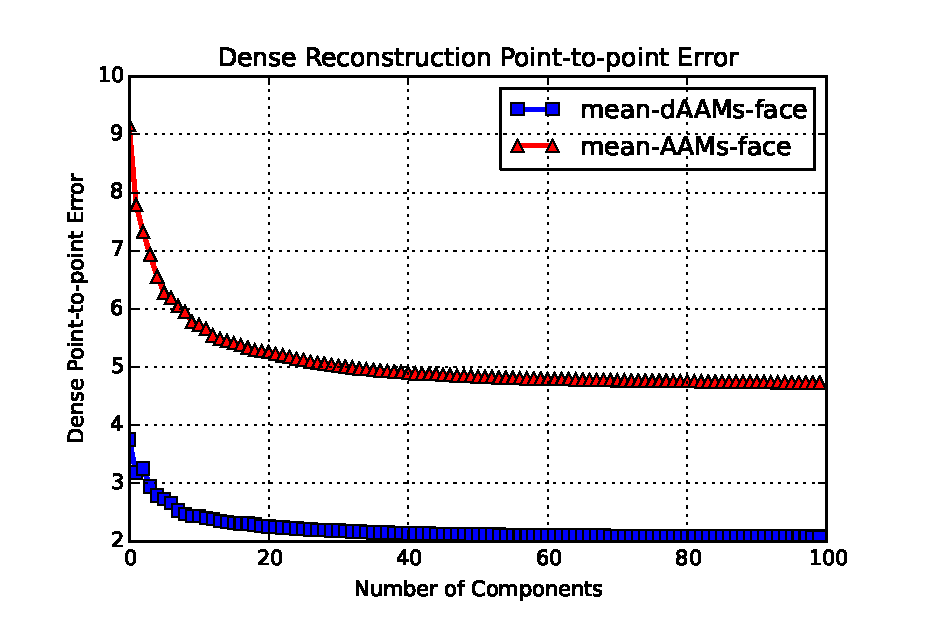
\includegraphics[width=\textwidth]{Suplementory_Meterial/Model_Analysis/sr_face}
        %\caption{AAMs dense shape reconstruction}
    \end{subfigure}
    \caption{Dense shape reconstruction errors for ears and faces. Top: results of reconstruction on ears, bottom: results of reconstruction on faces. The normalised point-to-point error is used an evaluation measure.}
    \label{fig:rc_face}
\end{figure}


We first investigate the reconstruction accuracy of AAMs and dAAMs in the shape space. In particular, given a ground-truth shape, we use the shape models from both AAMs and dAAMs to reconstruct the given shape densely. Since AAMs contain a sparse shape model, we densify it using a piecewise affine transformation, which is typically used in warping textures on to shape model too. Figure \ref{fig:rc_face} shows plots of dense shape reconstruction errors for ears and faces, for varying number of principal components kept. We observe that dAAMs significantly outperform classic AAMs on shape reconstruction.


Furthermore, we explore the compactness of the built AAMs and dAAMs models.
Figure \ref{fig:compact} demonstrates the variance explained as a function of the number of principal components. One can infer that dAAMs have a more compact shape model than AAMs, which leads to better reconstruction especially with few shape components.

\begin{figure}[!b]
    \centering
    \begin{subfigure}[b]{0.43\textwidth}
            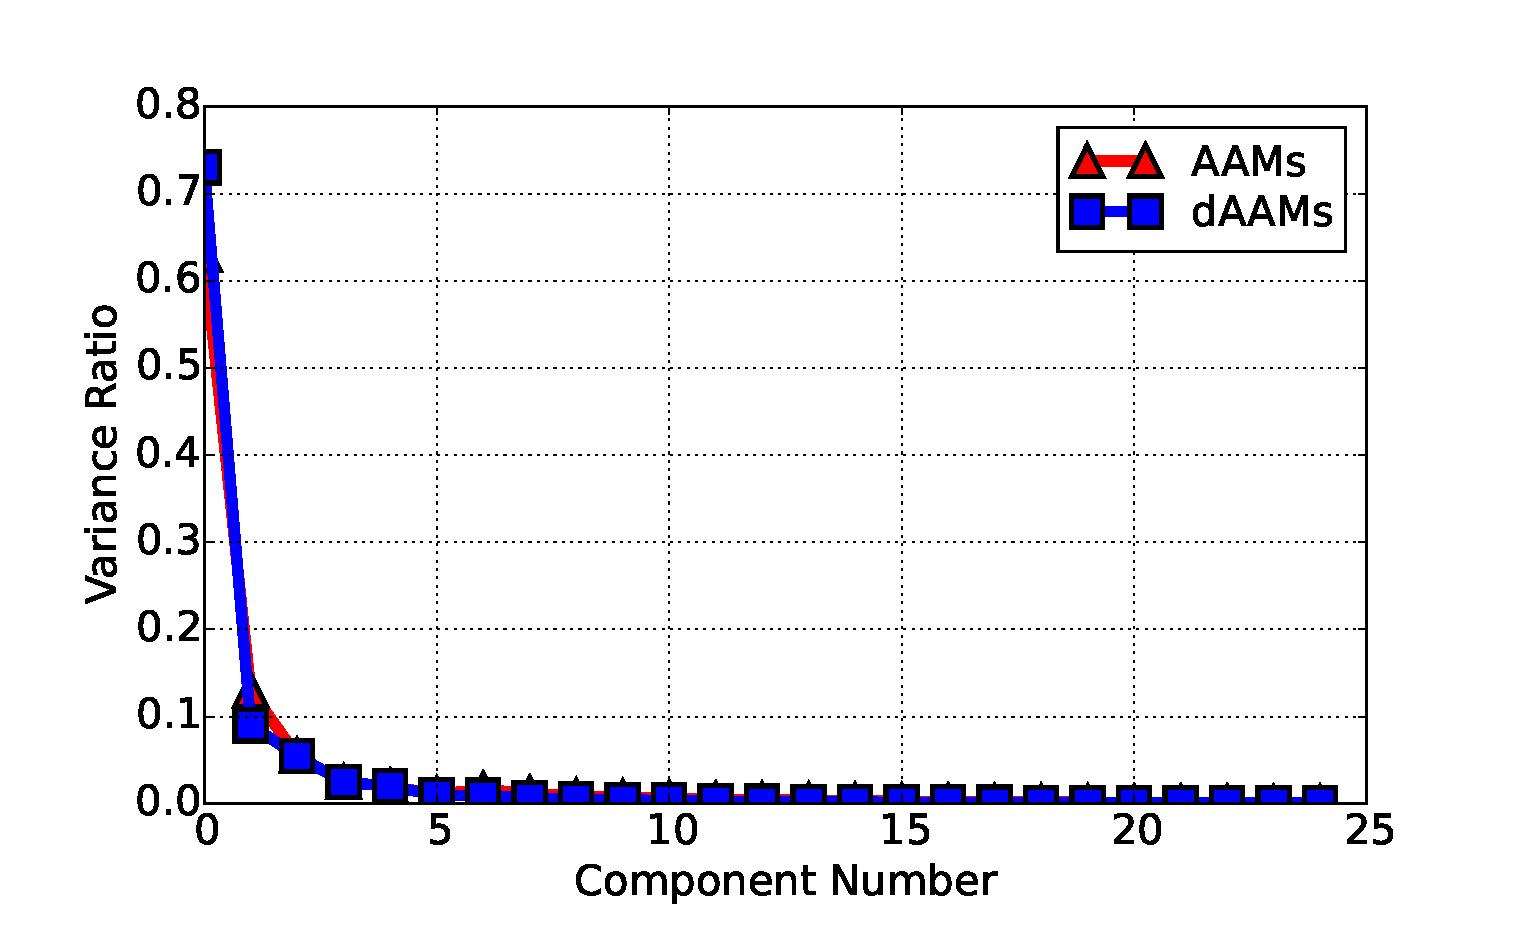
\includegraphics[width=\textwidth]{Suplementory_Meterial/Model_Analysis/var_ratio}
        %\caption{dAAMs vs AAMs Variance Ratio}
    \end{subfigure}
    \begin{subfigure}[b]{0.43\textwidth}
            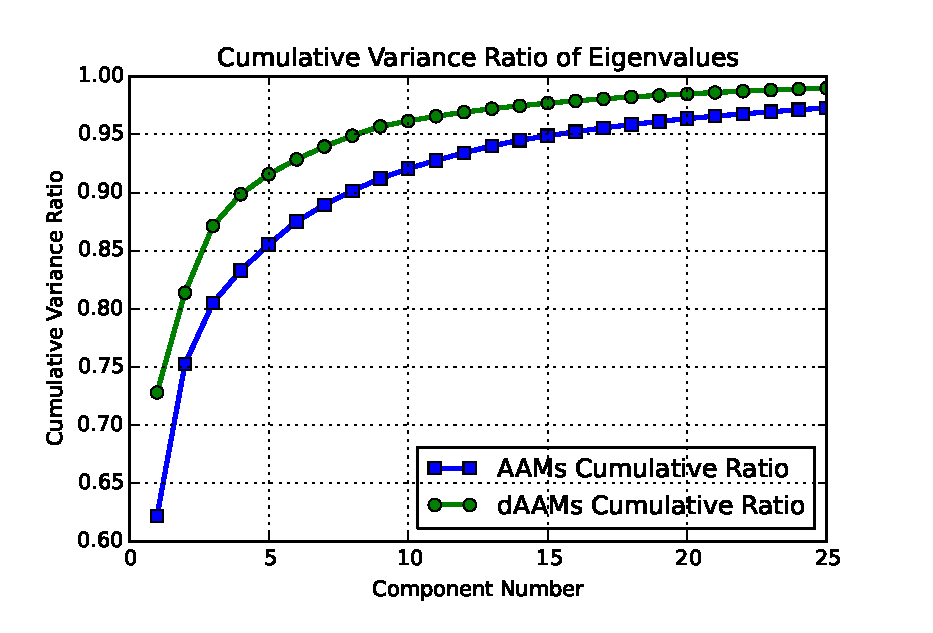
\includegraphics[width=\textwidth]{Suplementory_Meterial/Model_Analysis/cumu_var_ratio}
        %\caption{dAAMs vs AAMs Cumulative Variance Ratio}
    \end{subfigure}
    \caption{Variance explained by each principal component, for both dAAM and AAM models. Top: variance explained by each principal component. Bottom: cumulative plot of the variance explained as a function of the principal components.}
    \label{fig:compact}
\end{figure}

Finally, Figure \ref{fig:pcamodel} visualises the principal components of dAAMs for ears and faces. We observe that the variation of both shape and appearance captured by the model seem plausible.














\section{Patch-based Active Appearance Model}
\label{sec:paam}


\begin{figure*}[!t]
    \newcommand{\ofh}{0.24\columnwidth}
    \centering
    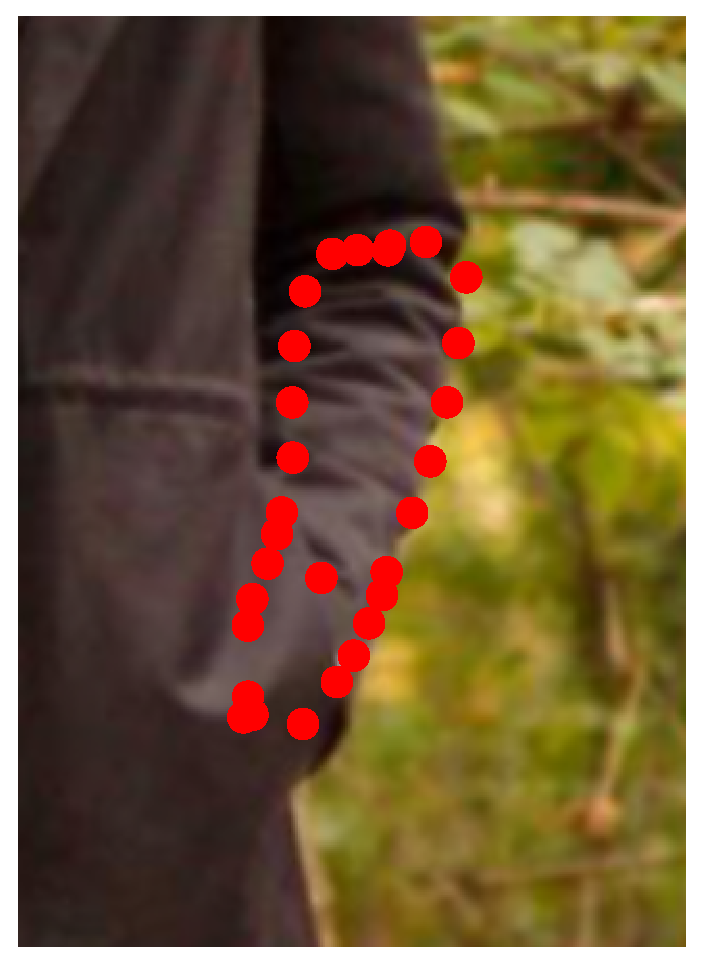
\includegraphics[height=\ofh]{Suplementory_Meterial/ExFit/0001.eps}
    \hfill
    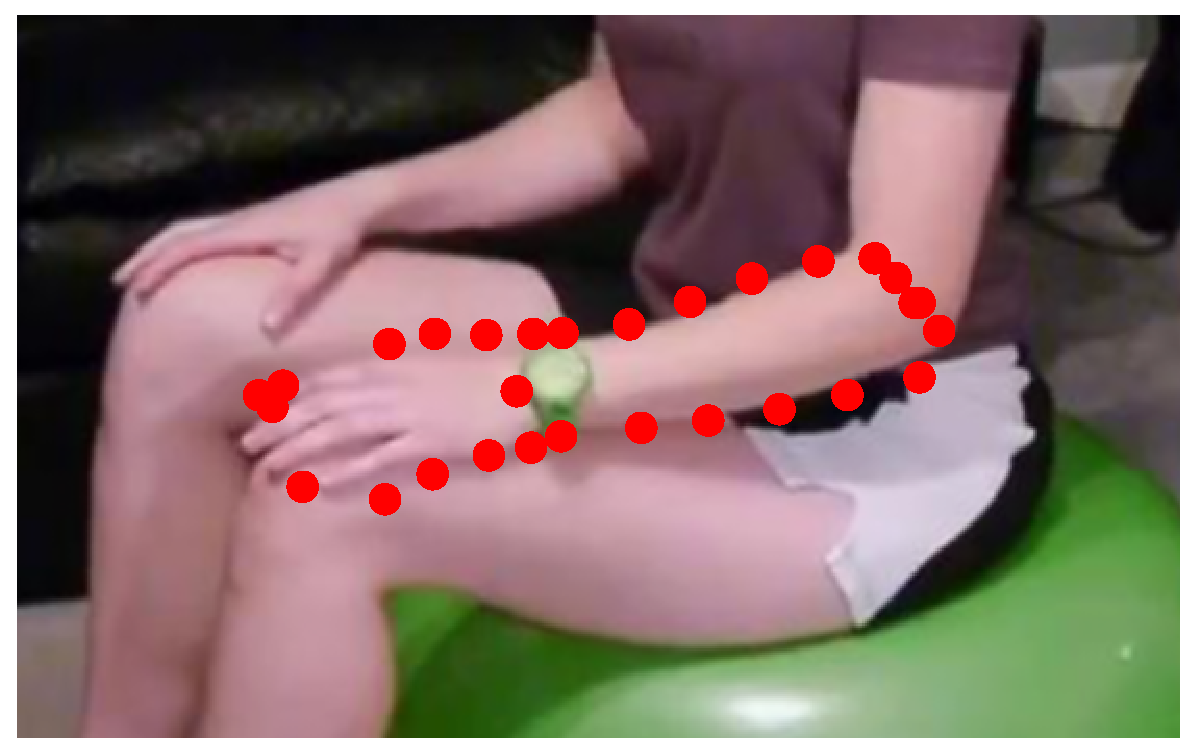
\includegraphics[height=\ofh]{Suplementory_Meterial/ExFit/0002.eps}
    \hfill
    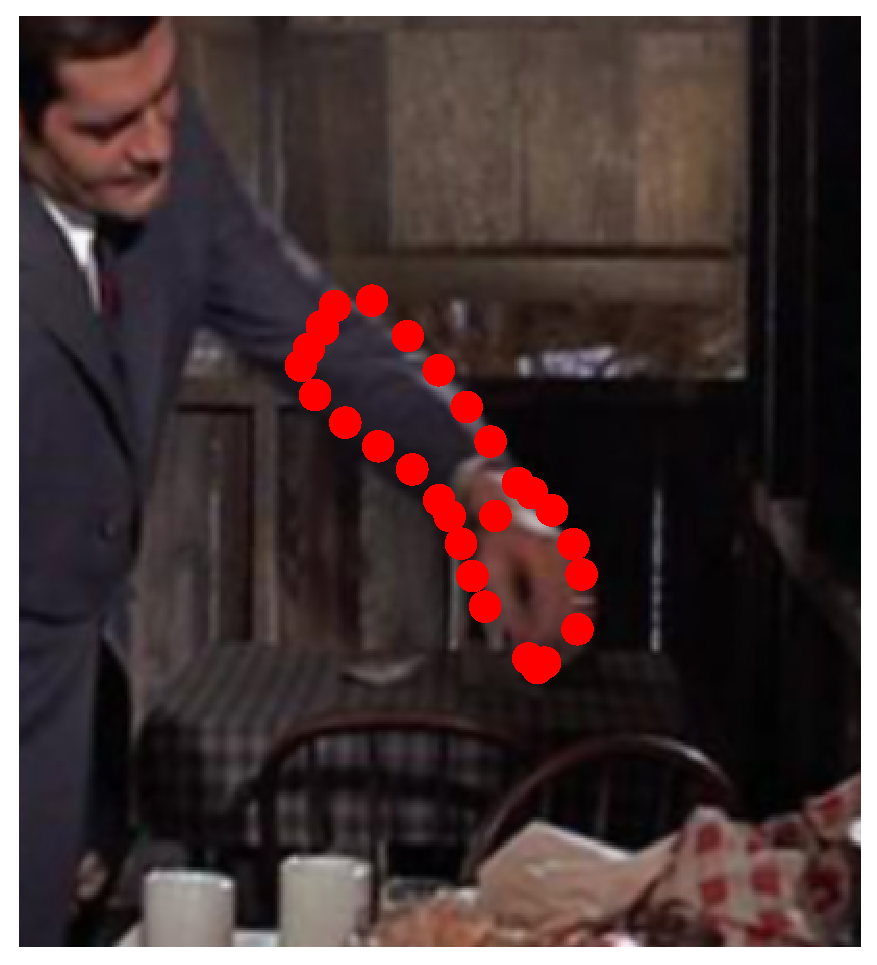
\includegraphics[height=\ofh]{Suplementory_Meterial/ExFit/0003.eps}
    \hfill
    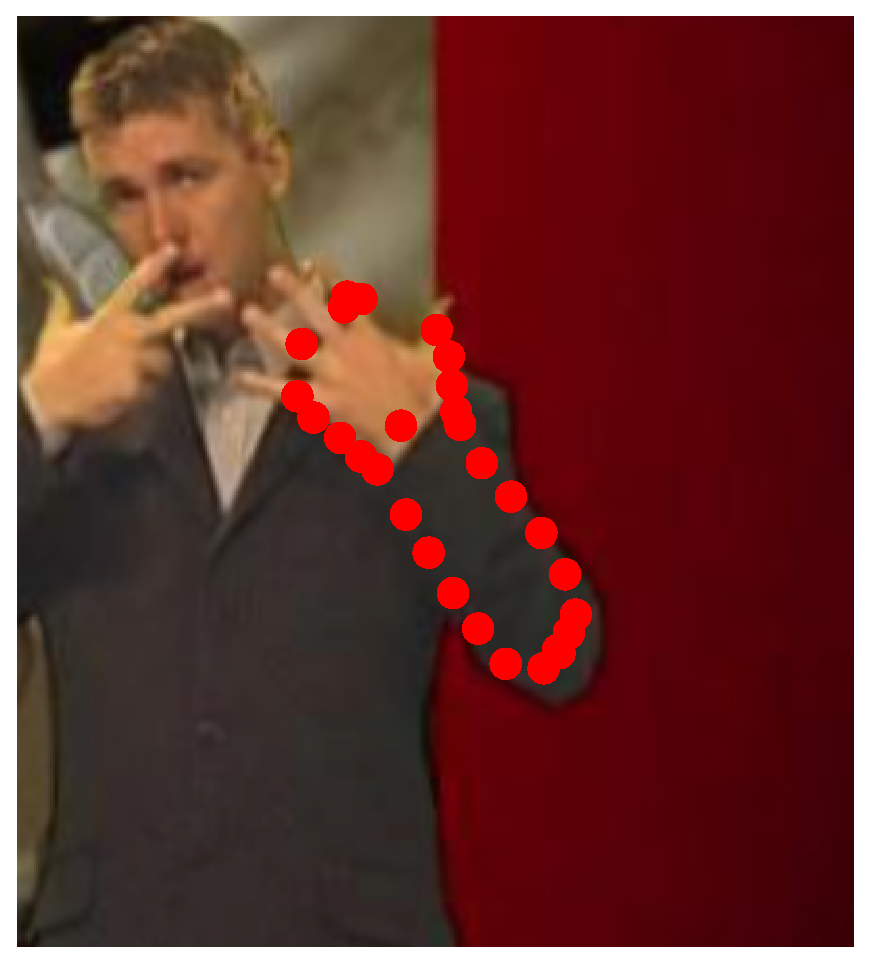
\includegraphics[height=\ofh]{Suplementory_Meterial/ExFit/0004.eps}
    \hfill
    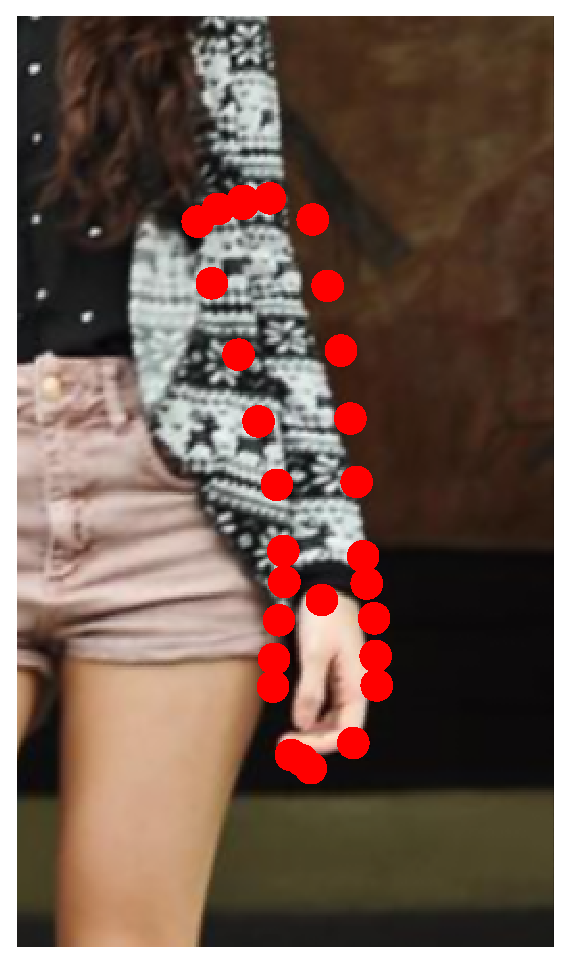
\includegraphics[height=\ofh]{Suplementory_Meterial/ExFit/0005.eps}
    \hfill
    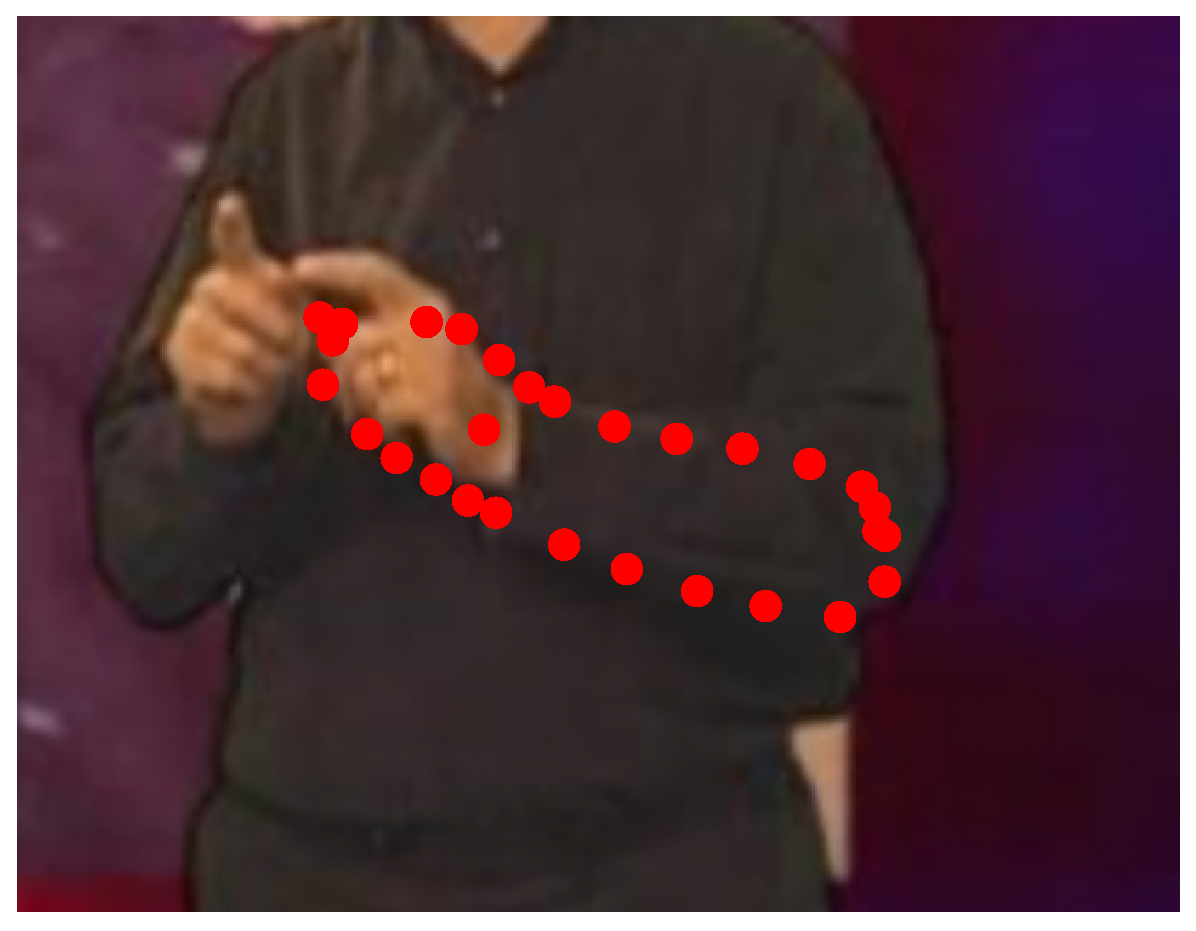
\includegraphics[height=\ofh]{Suplementory_Meterial/ExFit/0006.eps}
    \hfill
    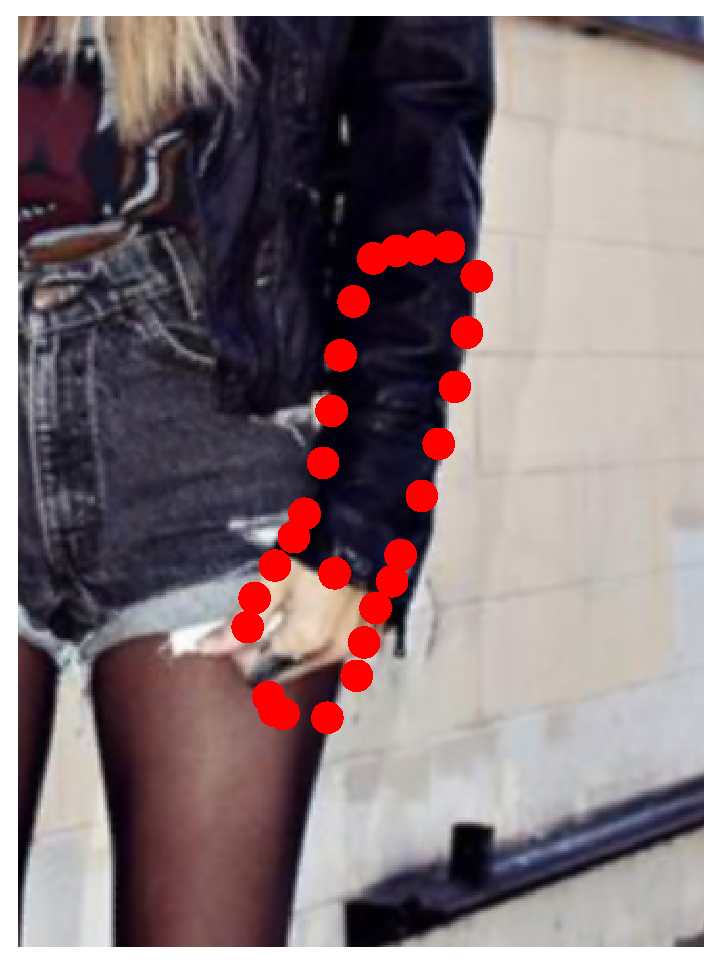
\includegraphics[height=\ofh]{Suplementory_Meterial/ExFit/0007.eps}
    \hfill
    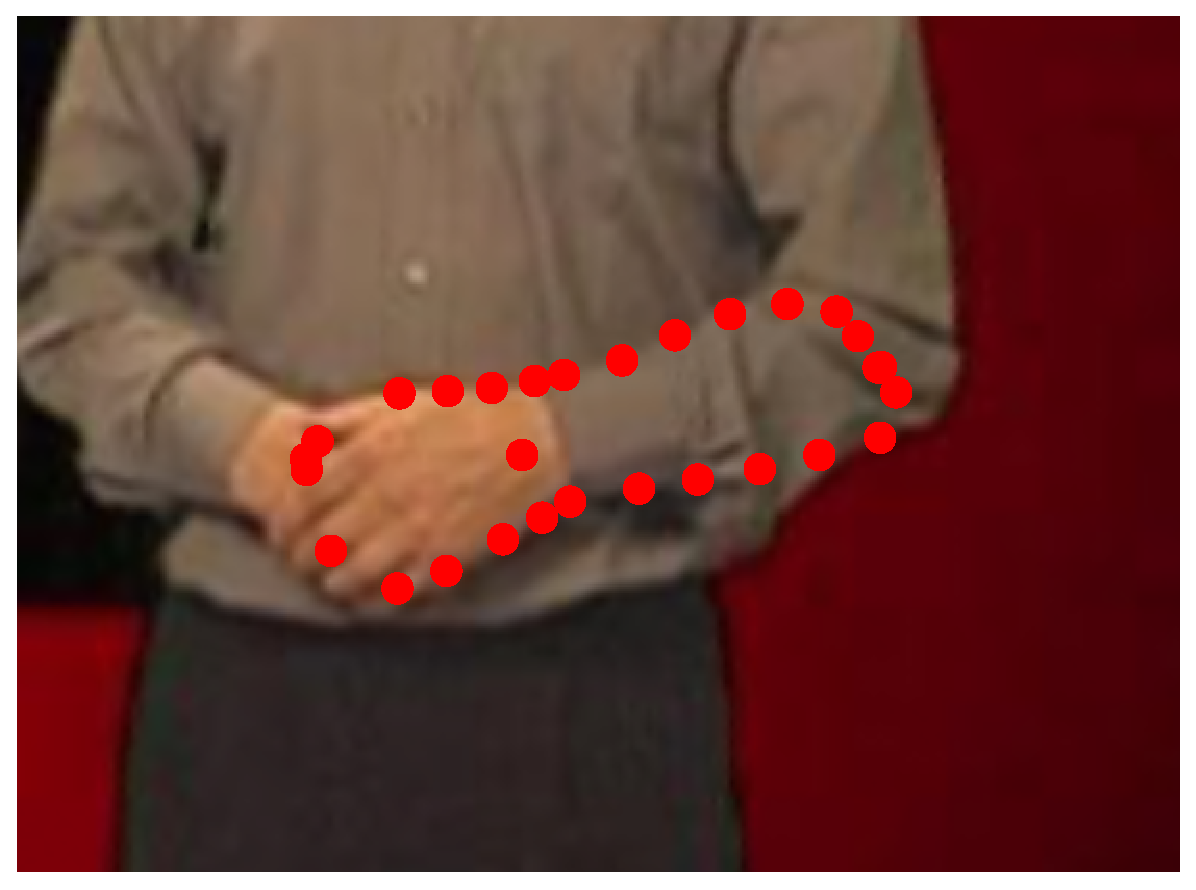
\includegraphics[height=\ofh]{Suplementory_Meterial/ExFit/0008.eps}
    \hfill
    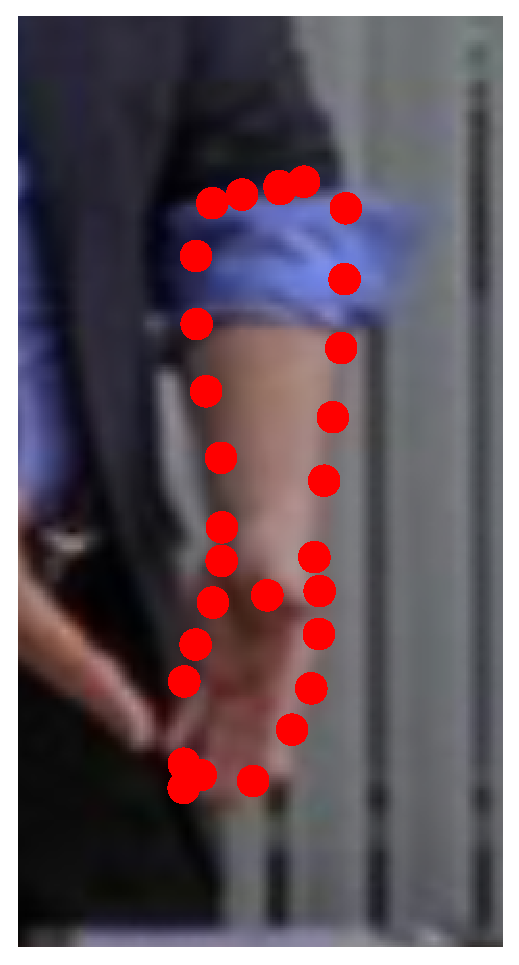
\includegraphics[height=\ofh]{Suplementory_Meterial/ExFit/0009.eps}
    \hfill
    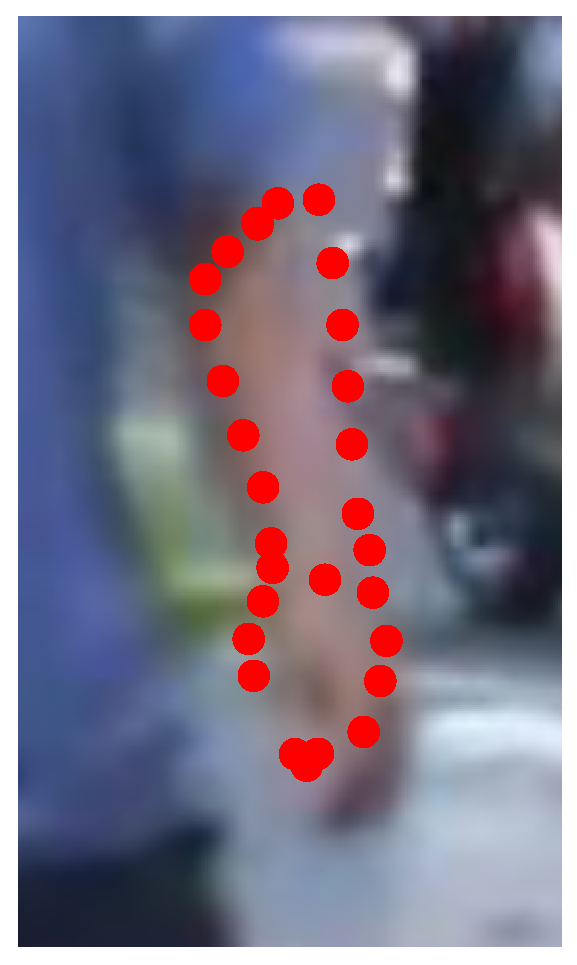
\includegraphics[height=\ofh]{Suplementory_Meterial/ExFit/0010.eps}
    \hfill
    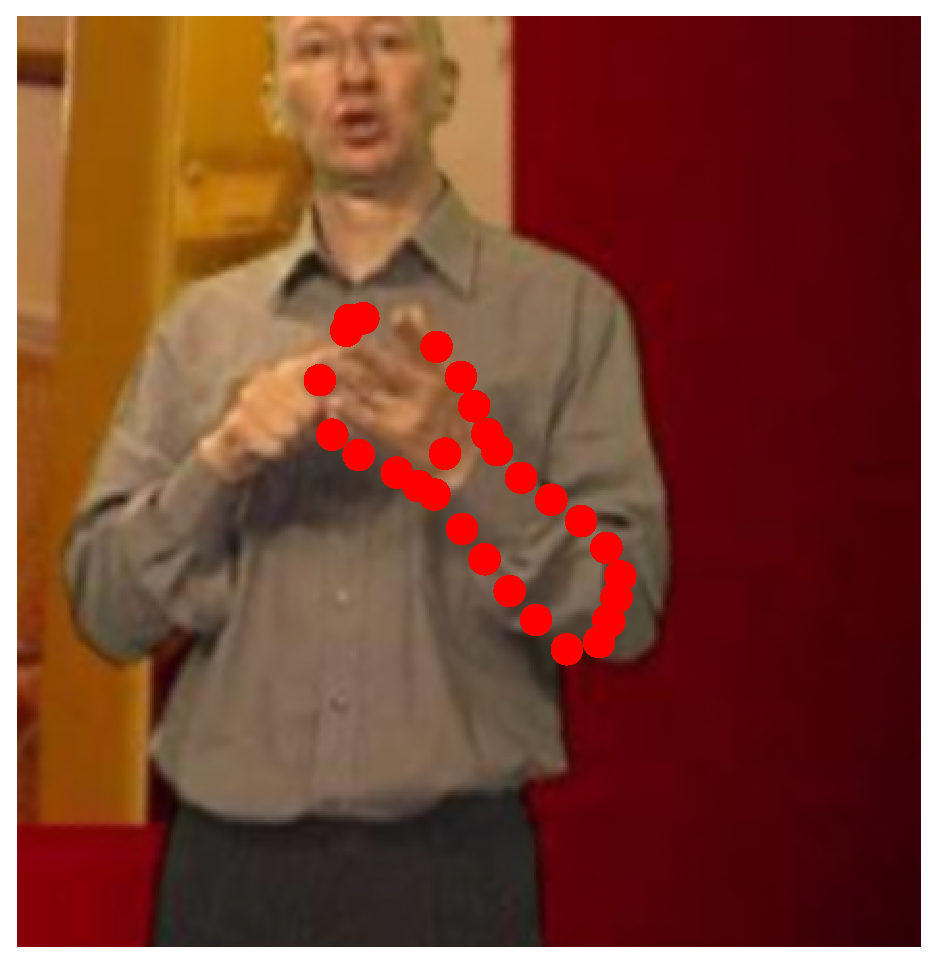
\includegraphics[height=\ofh]{Suplementory_Meterial/ExFit/0011.eps}
    \hfill
    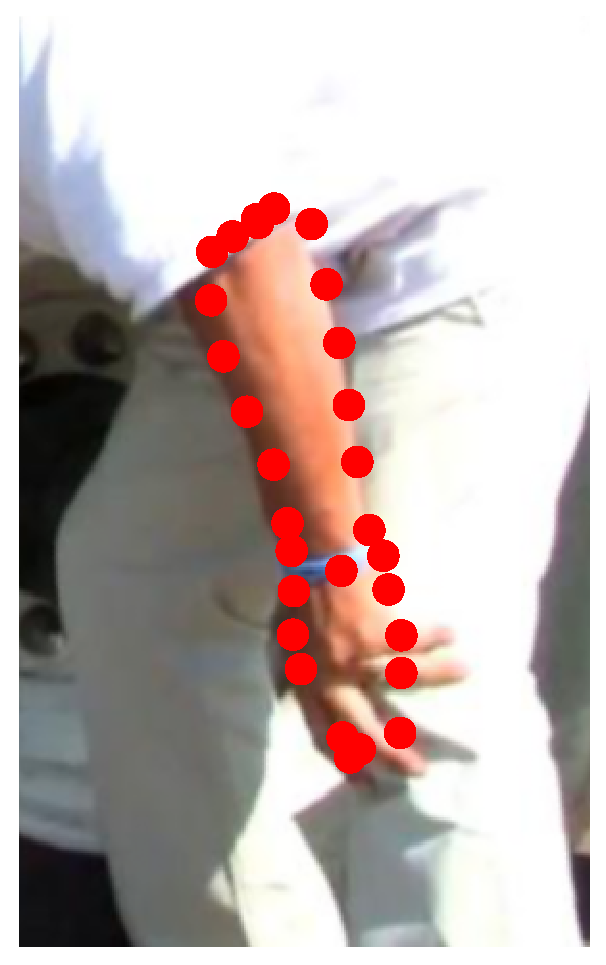
\includegraphics[height=\ofh]{Suplementory_Meterial/ExFit/0012.eps}
    \hfill
    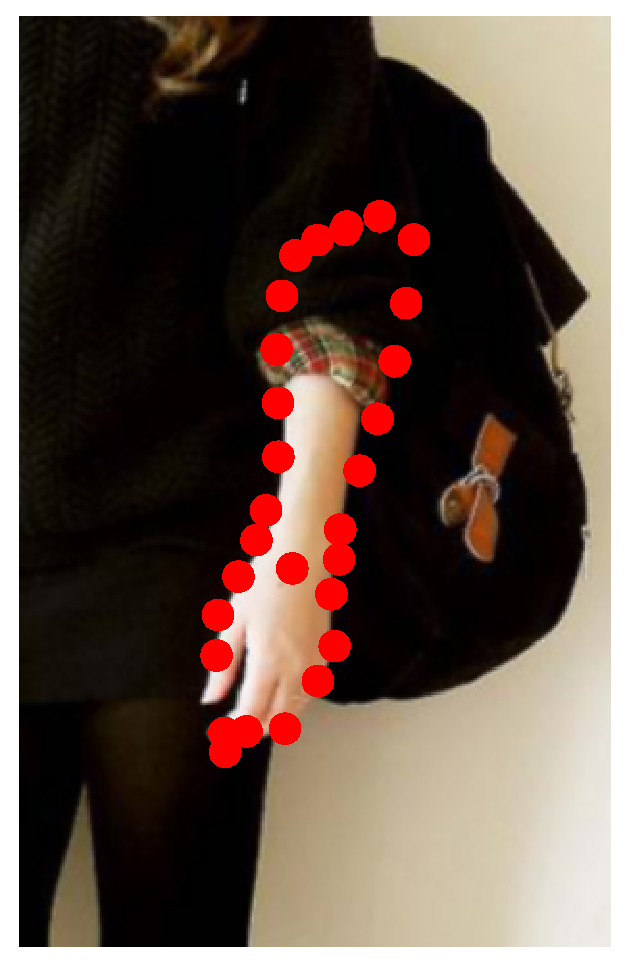
\includegraphics[height=\ofh]{Suplementory_Meterial/ExFit/0013.eps}
    \hfill
    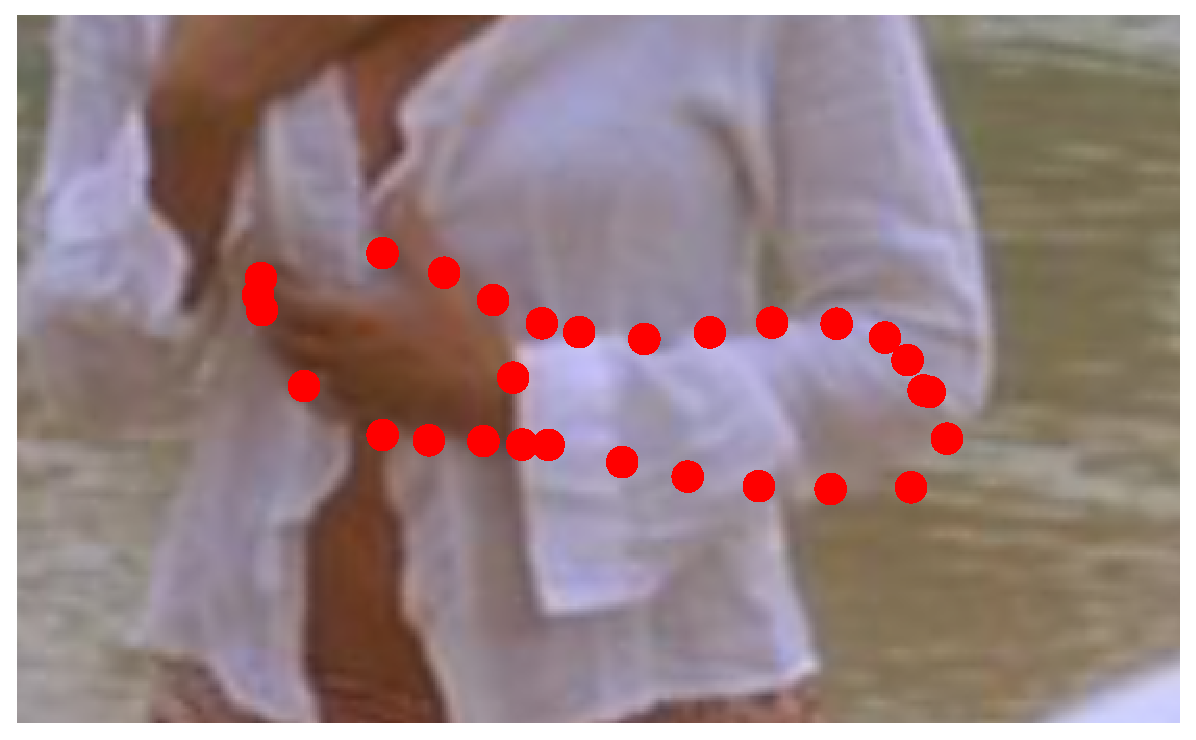
\includegraphics[height=\ofh]{Suplementory_Meterial/ExFit/0014.eps}
    \hfill
    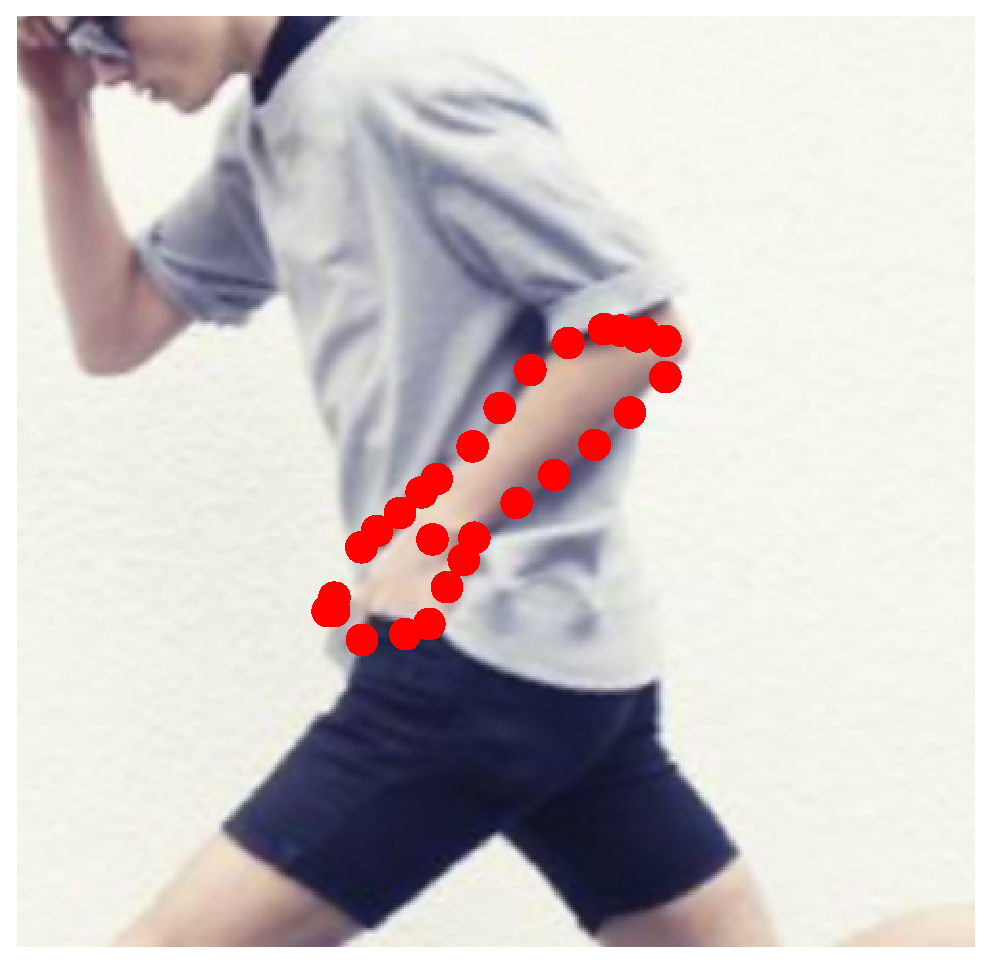
\includegraphics[height=\ofh]{Suplementory_Meterial/ExFit/0015.eps}
    \hfill
    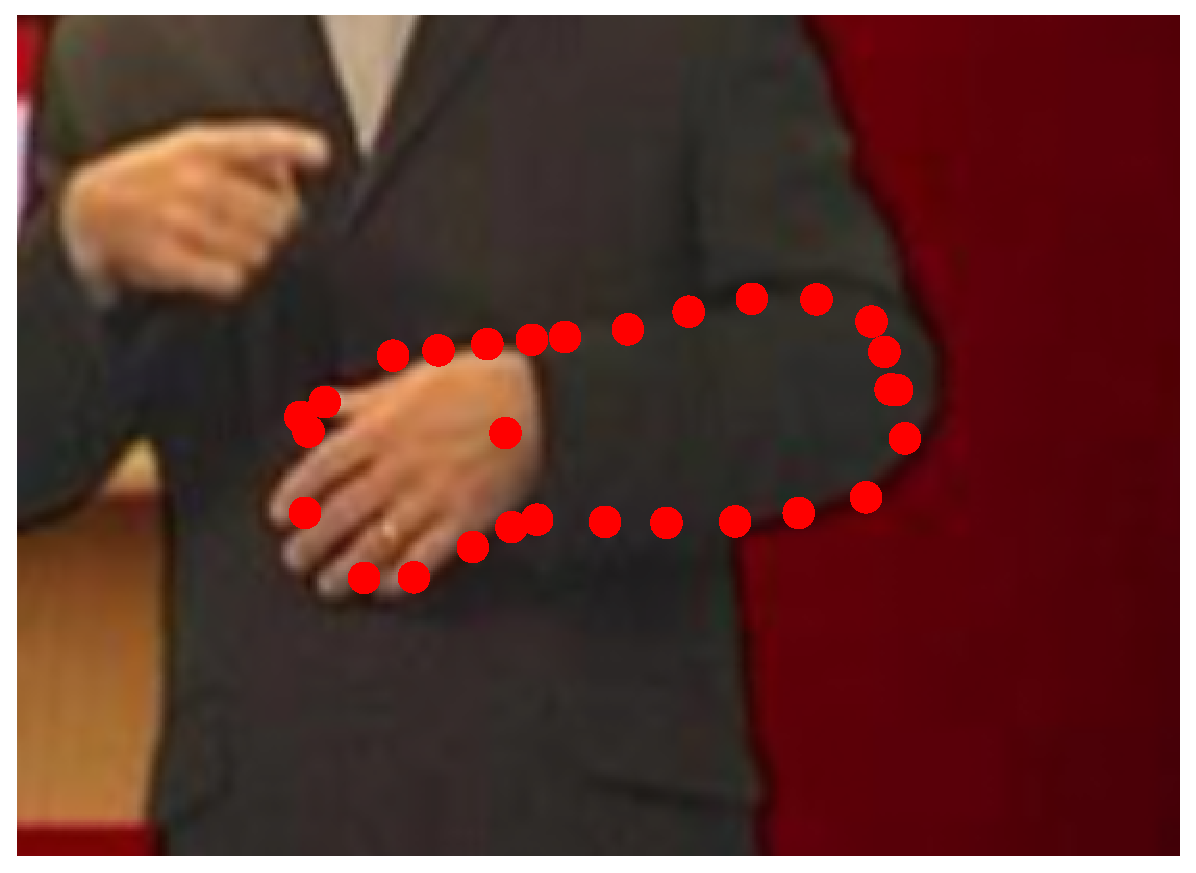
\includegraphics[height=\ofh]{Suplementory_Meterial/ExFit/0017.eps}
    \hfill
    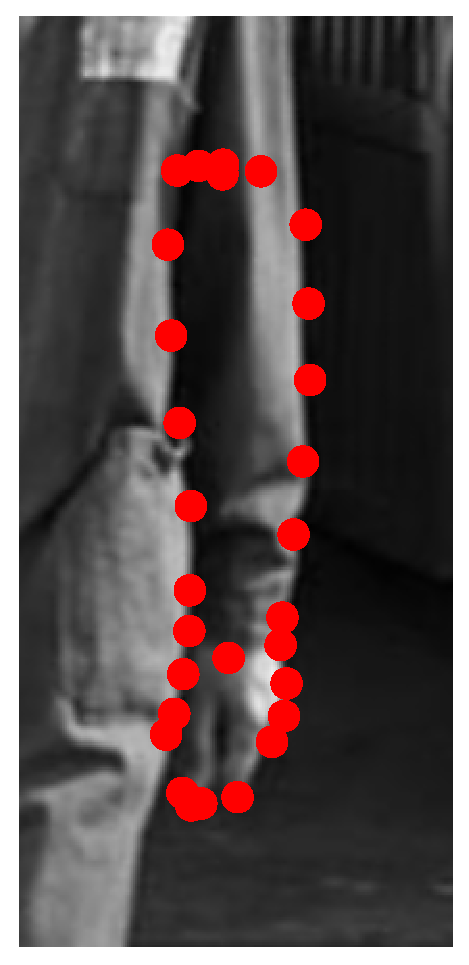
\includegraphics[height=\ofh]{Suplementory_Meterial/ExFit/0018.eps}
    \hfill
    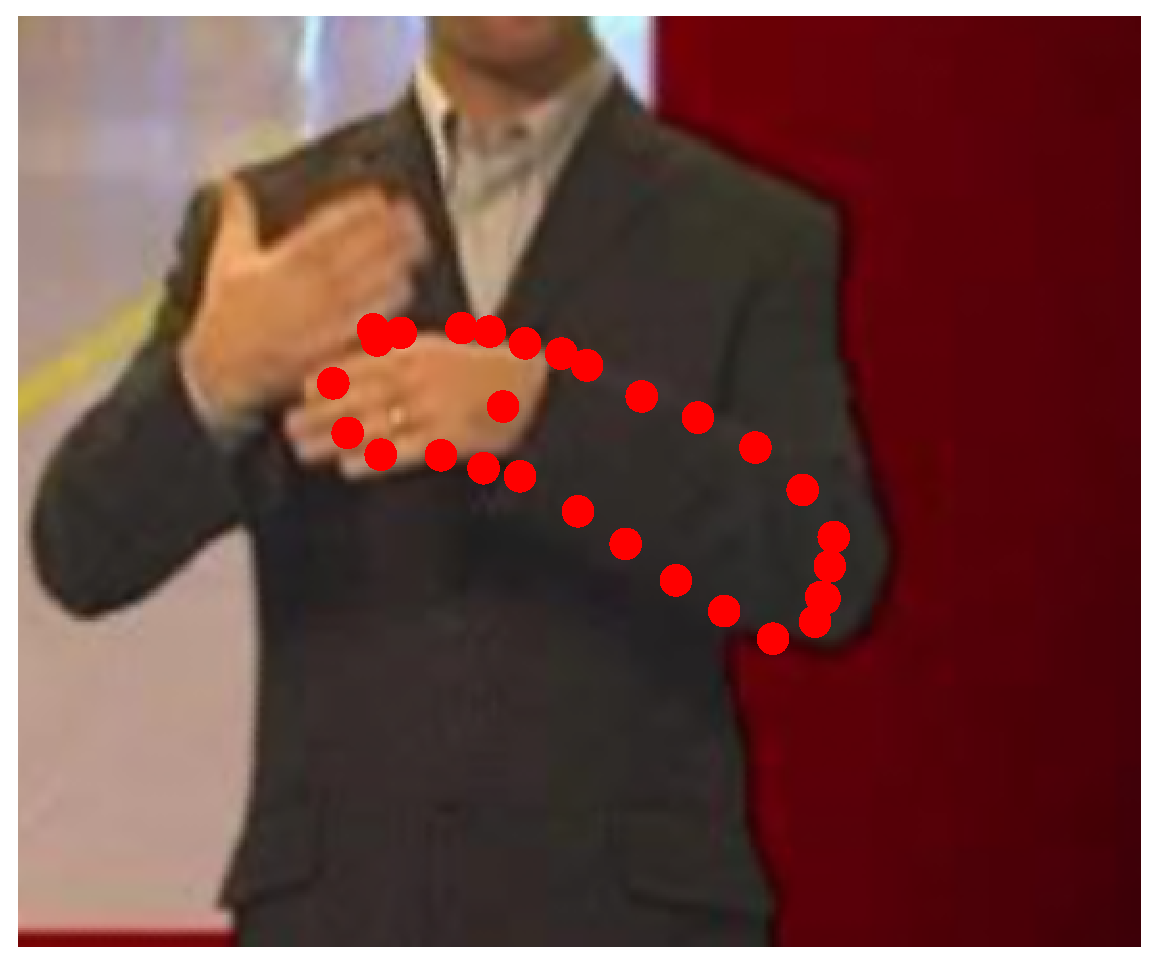
\includegraphics[height=\ofh]{Suplementory_Meterial/ExFit/0019.eps}
    \hfill
    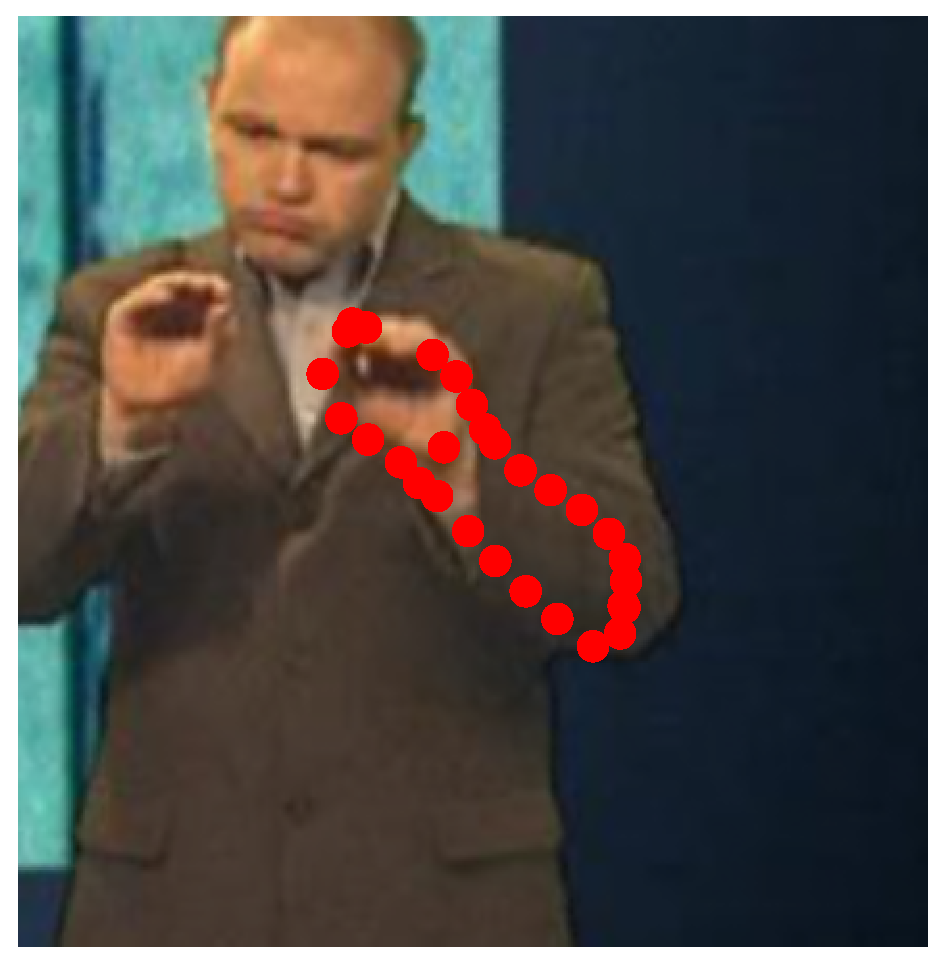
\includegraphics[height=\ofh]{Suplementory_Meterial/ExFit/0020.eps}
    \hfill
    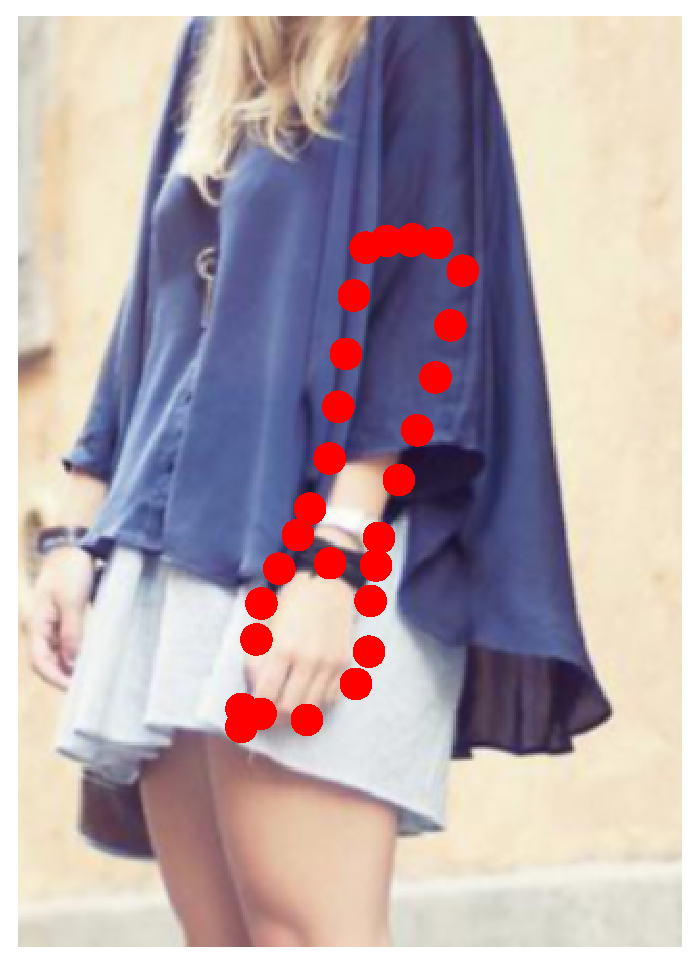
\includegraphics[height=\ofh]{Suplementory_Meterial/ExFit/0021.eps}
    \hfill
    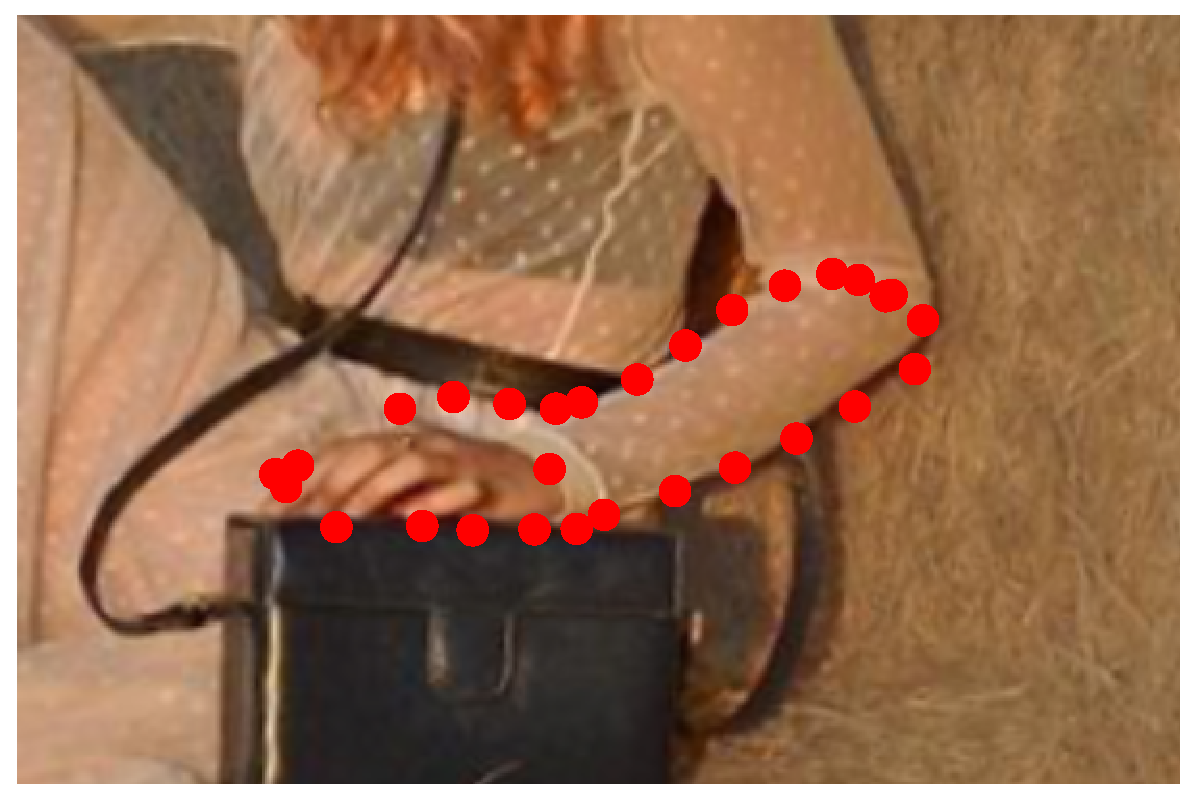
\includegraphics[height=\ofh]{Suplementory_Meterial/ExFit/0022.eps}
    \hfill
    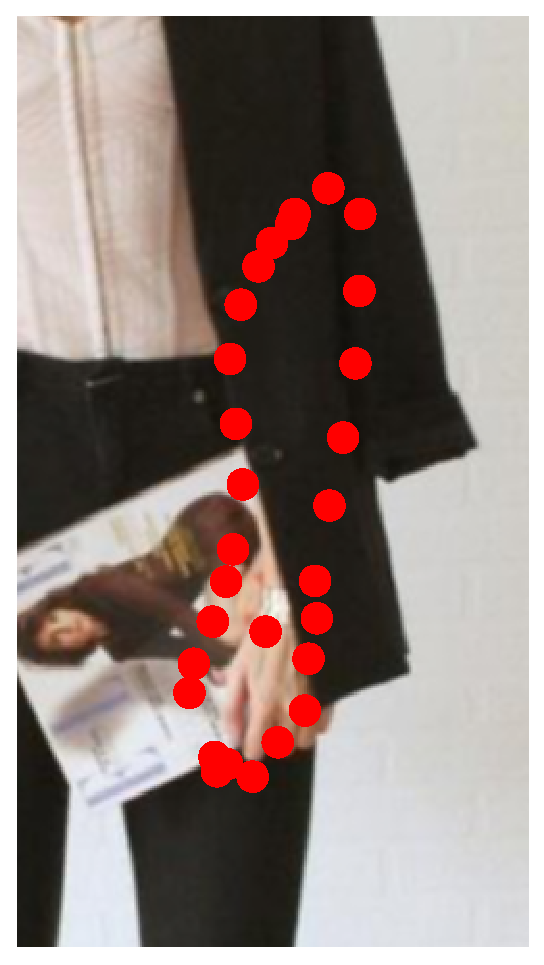
\includegraphics[height=\ofh]{Suplementory_Meterial/ExFit/0023.eps}
    \hfill
    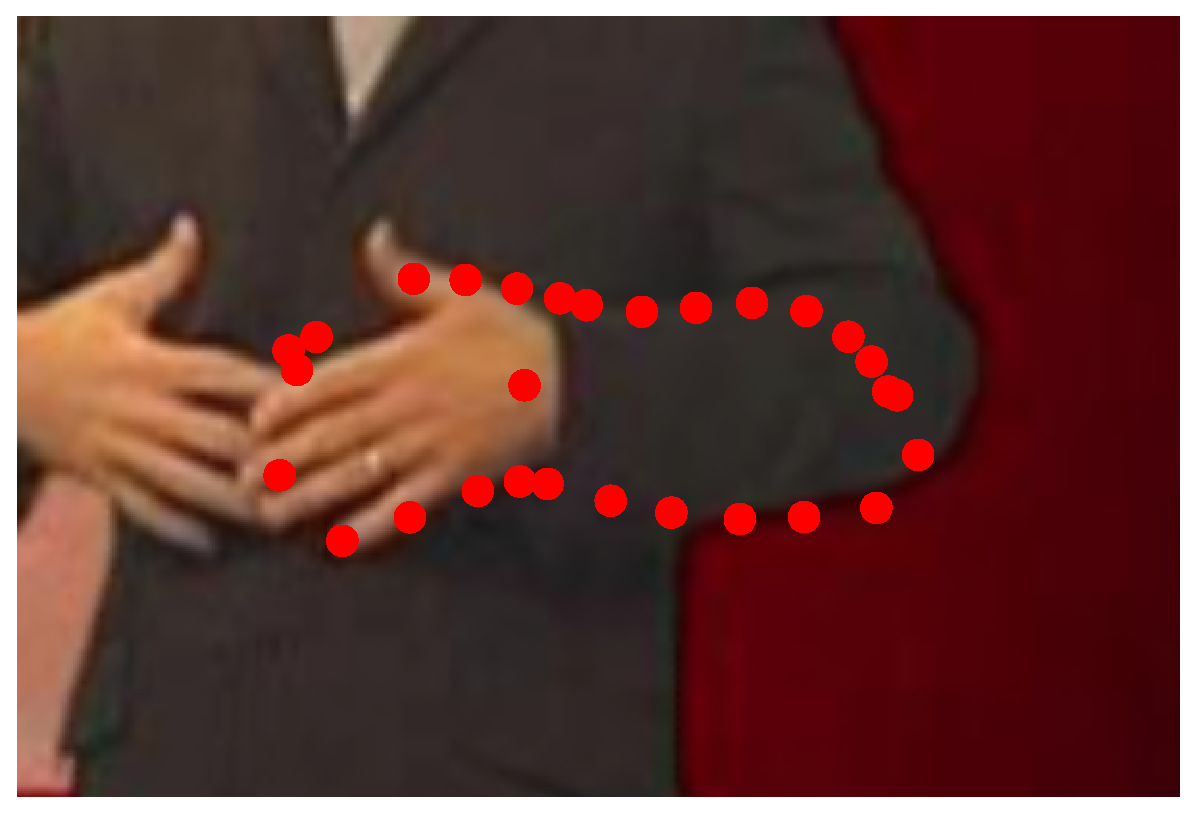
\includegraphics[height=\ofh]{Suplementory_Meterial/ExFit/0024.eps}
    \hfill
    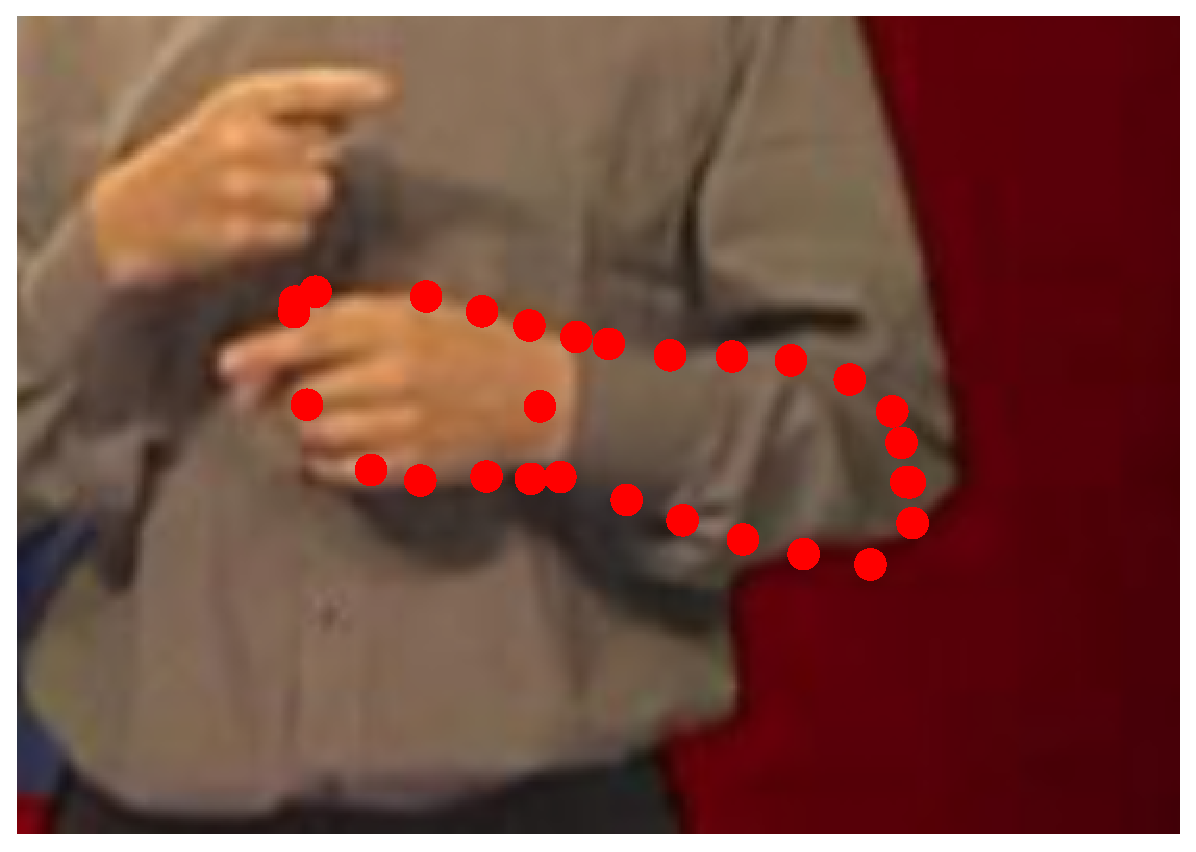
\includegraphics[height=\ofh]{Suplementory_Meterial/ExFit/0025.eps}
    \hfill
    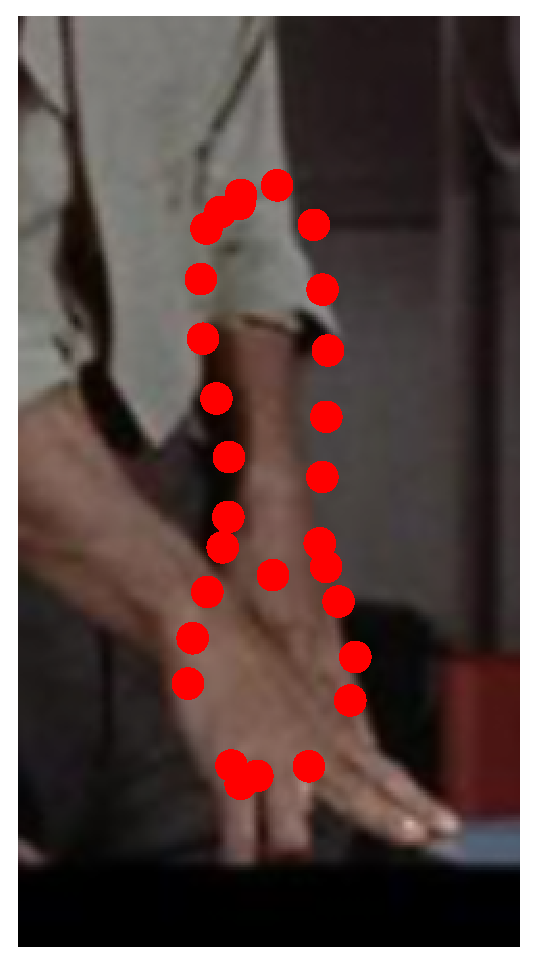
\includegraphics[height=\ofh]{Suplementory_Meterial/ExFit/0026.eps}
    \hfill
    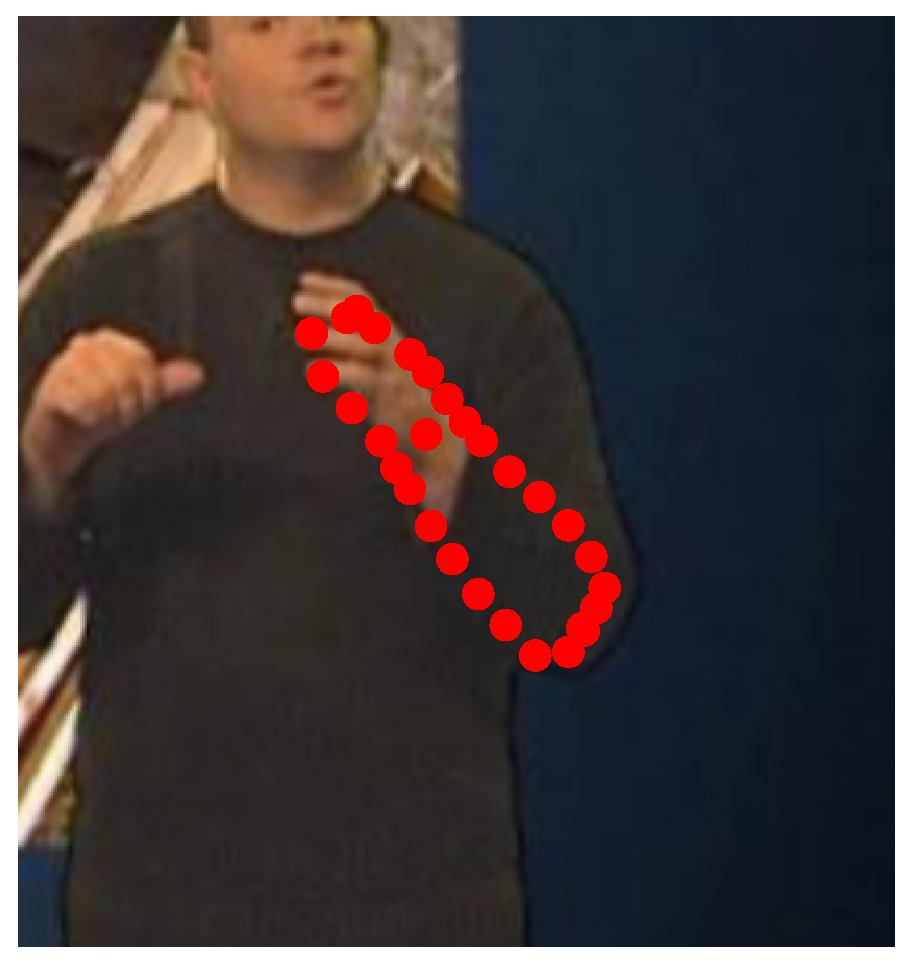
\includegraphics[height=\ofh]{Suplementory_Meterial/ExFit/0027.eps}
    \hfill
    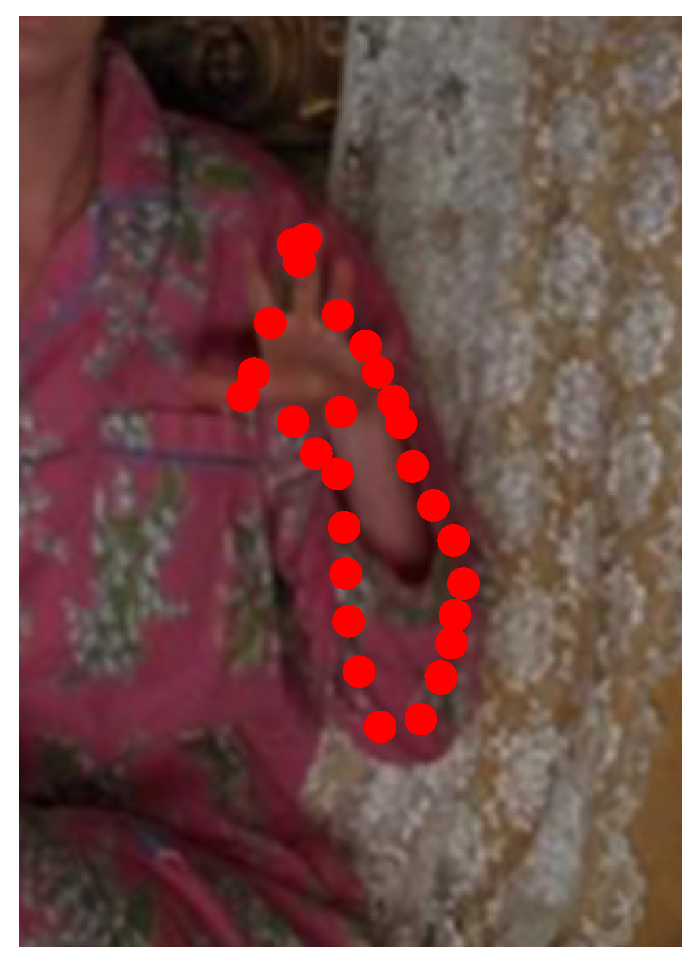
\includegraphics[height=\ofh]{Suplementory_Meterial/ExFit/0028.eps}
    \hfill
    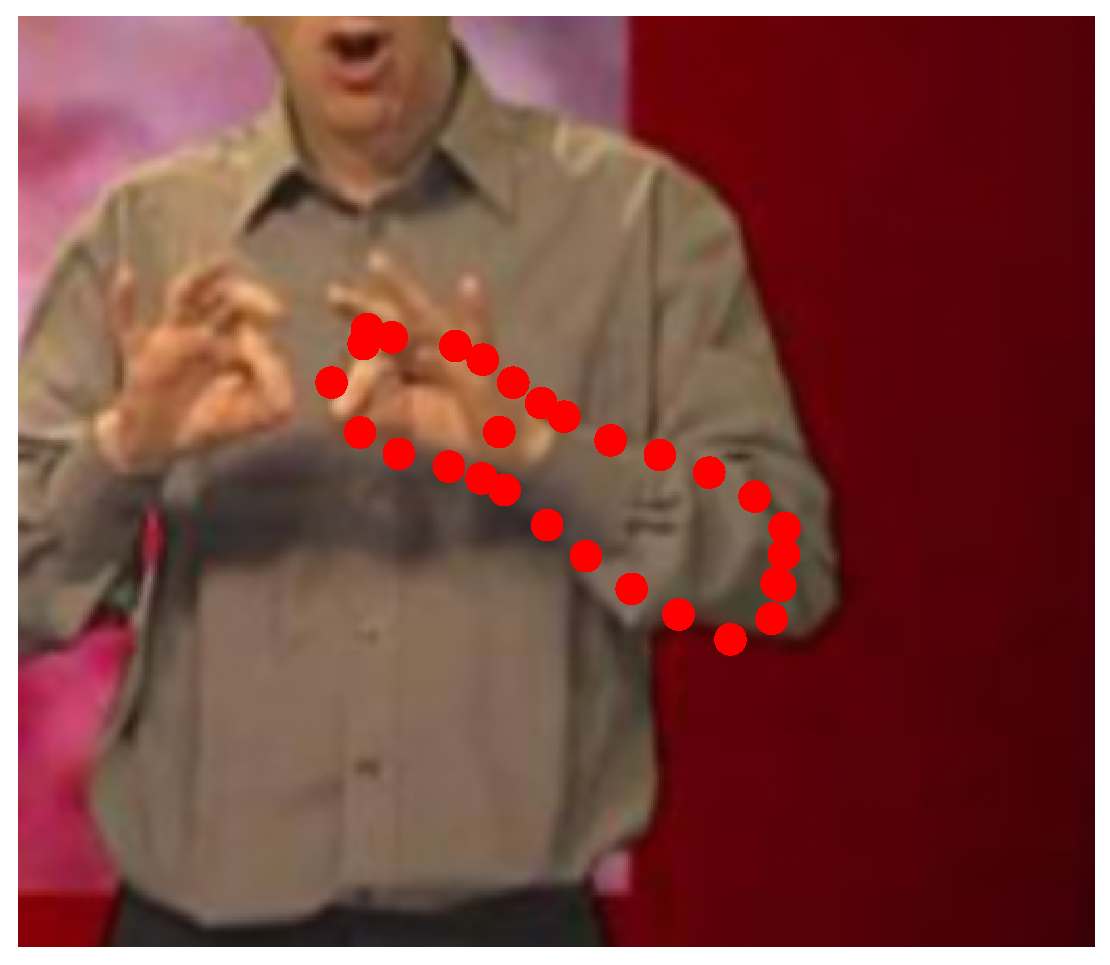
\includegraphics[height=\ofh]{Suplementory_Meterial/ExFit/0029.eps}
    \hfill
    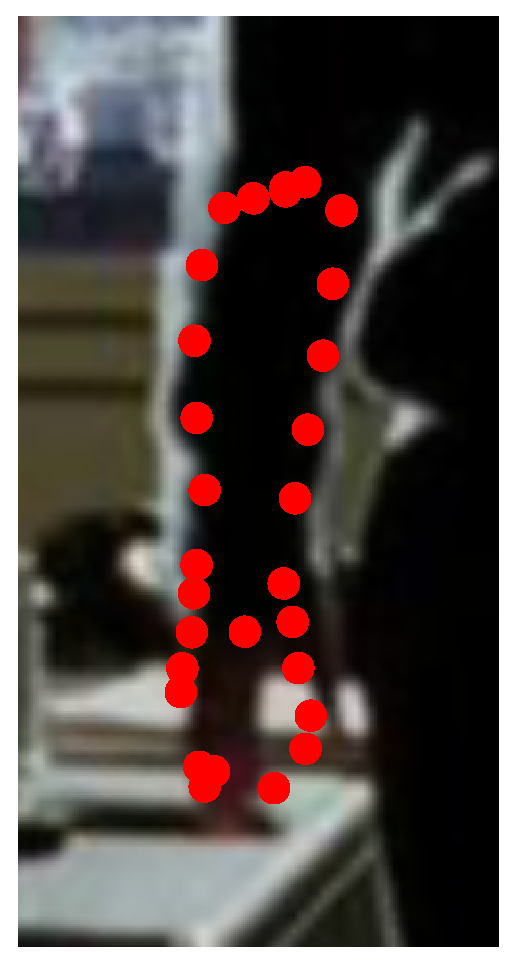
\includegraphics[height=\ofh]{Suplementory_Meterial/ExFit/0030.eps}
    \hfill
    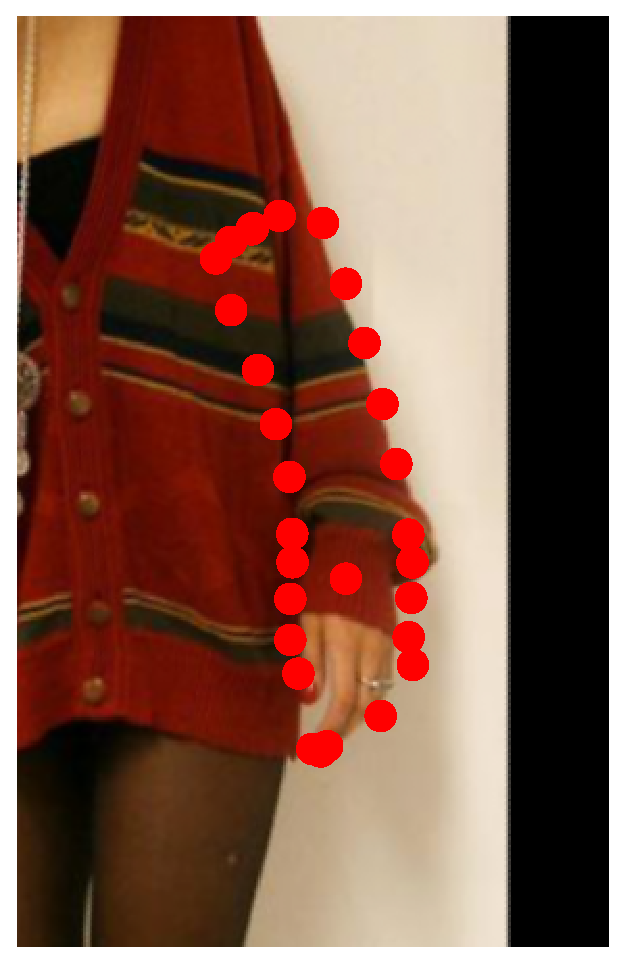
\includegraphics[height=\ofh]{Suplementory_Meterial/ExFit/0031.eps}
    \hfill
    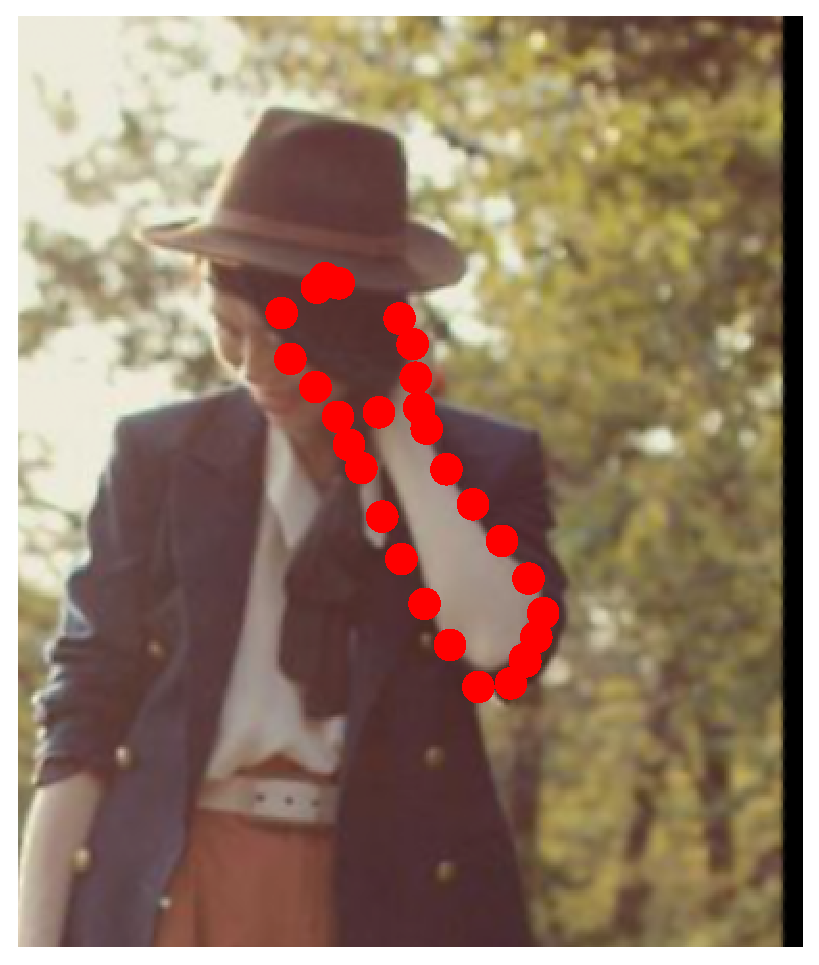
\includegraphics[height=\ofh]{Suplementory_Meterial/ExFit/0032.eps}
    \hfill
    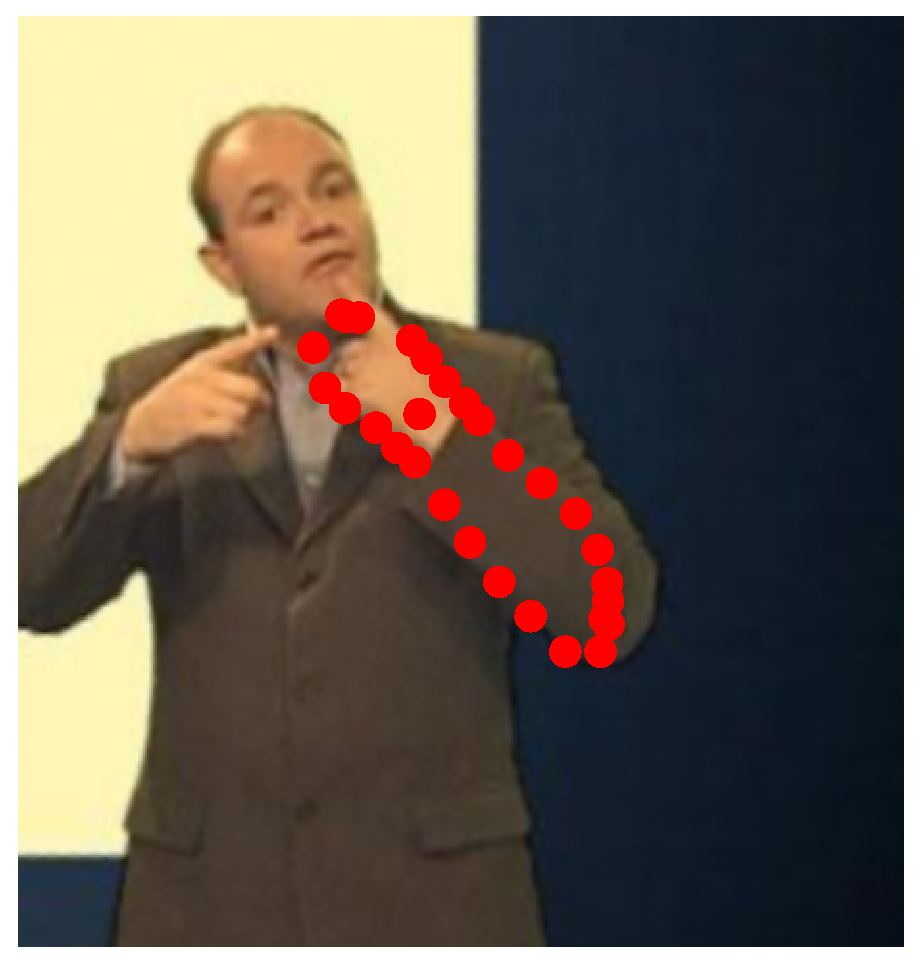
\includegraphics[height=\ofh]{Suplementory_Meterial/ExFit/0033.eps}
    \hfill
    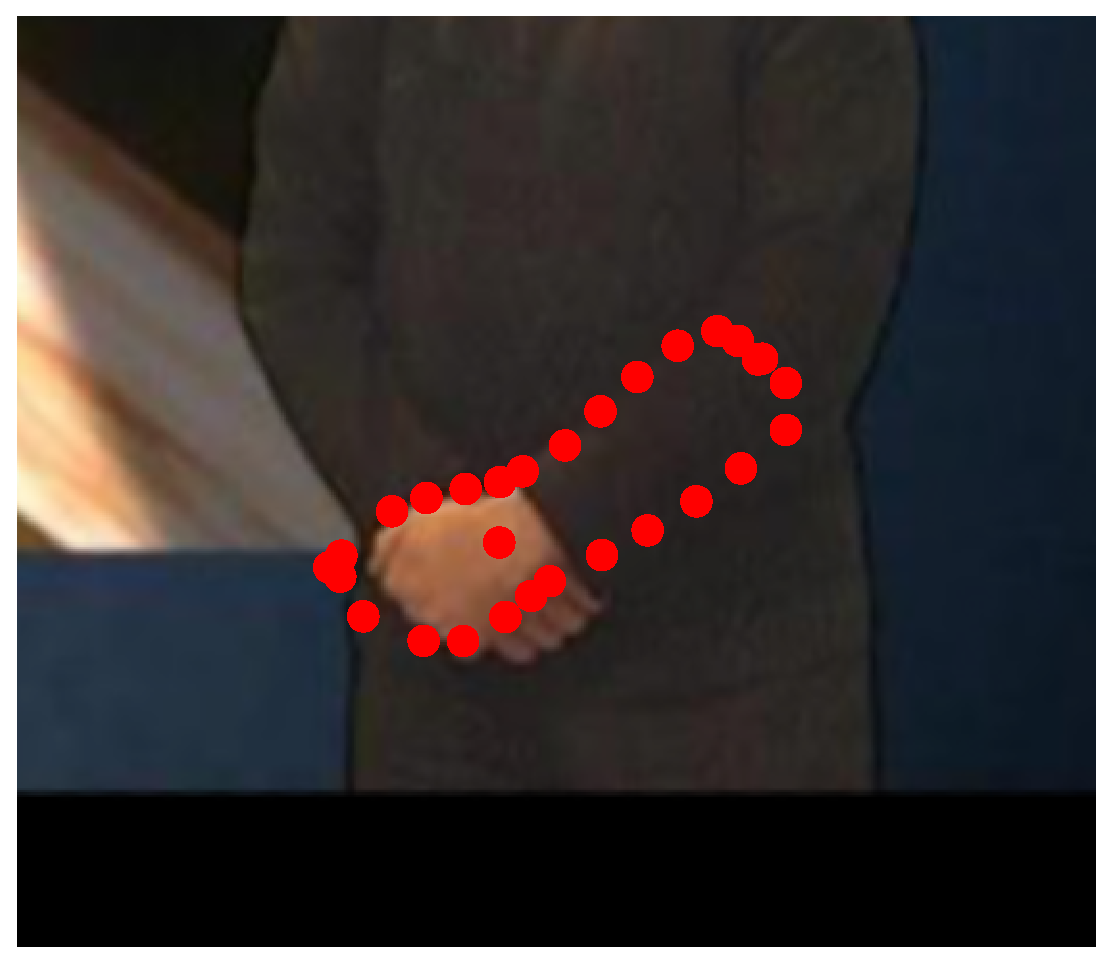
\includegraphics[height=\ofh]{Suplementory_Meterial/ExFit/0034.eps}
    \hfill
    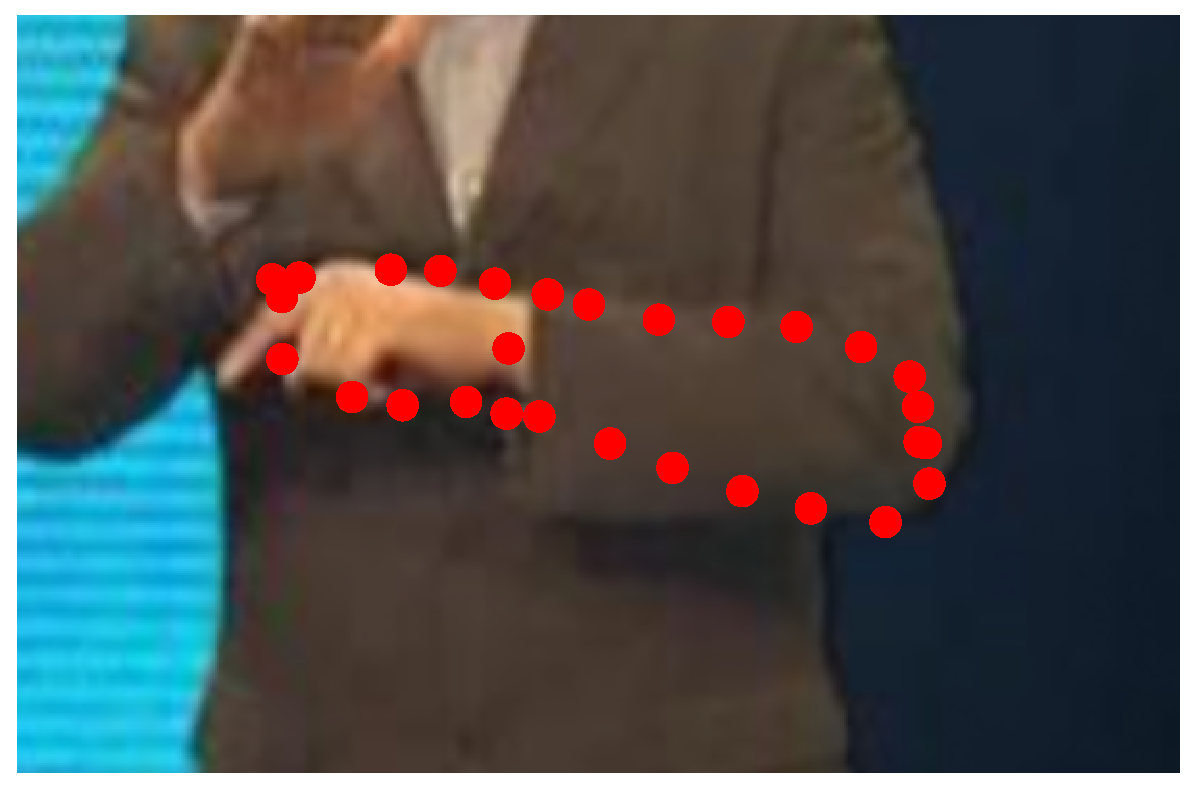
\includegraphics[height=\ofh]{Suplementory_Meterial/ExFit/0035.eps}
    \hfill
    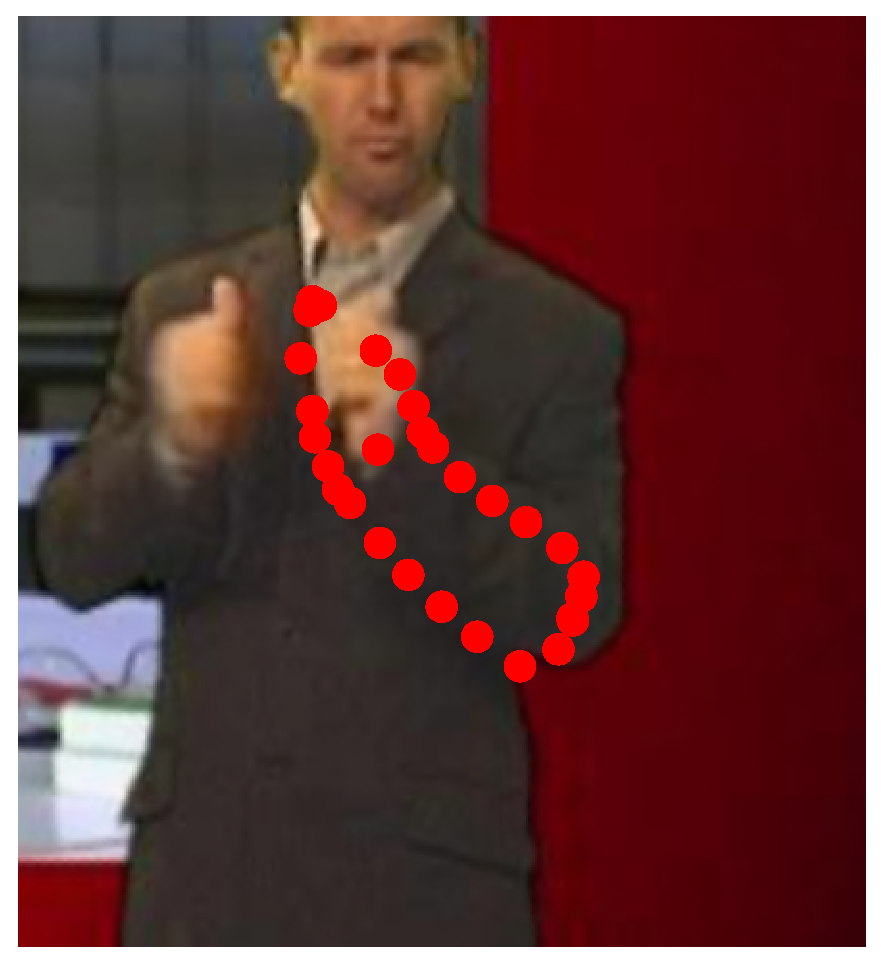
\includegraphics[height=\ofh]{Suplementory_Meterial/ExFit/0036.eps}
    \hfill
    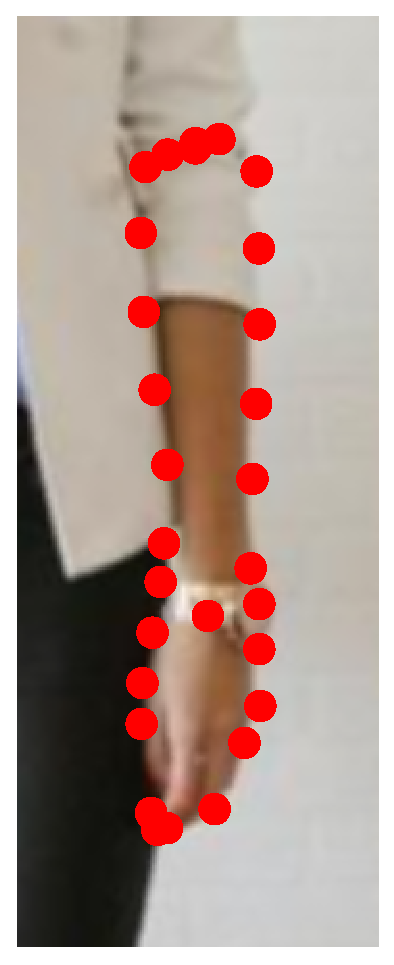
\includegraphics[height=\ofh]{Suplementory_Meterial/ExFit/0037.eps}
    \hfill
    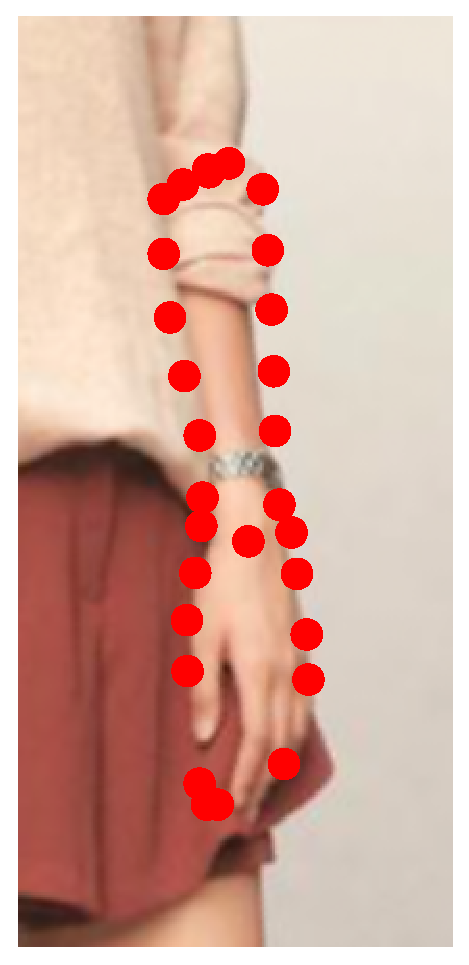
\includegraphics[height=\ofh]{Suplementory_Meterial/ExFit/0038.eps}
    \hfill
    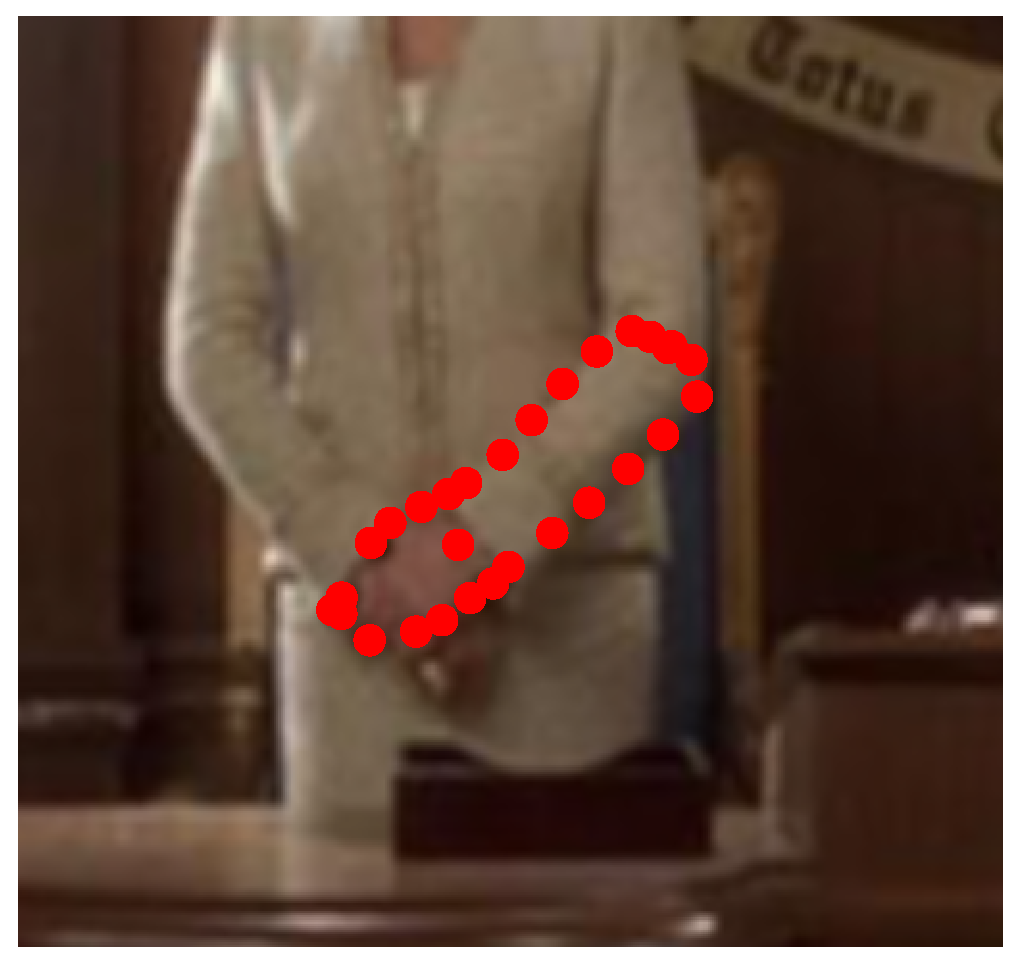
\includegraphics[height=\ofh]{Suplementory_Meterial/ExFit/0039.eps}
    \hfill
    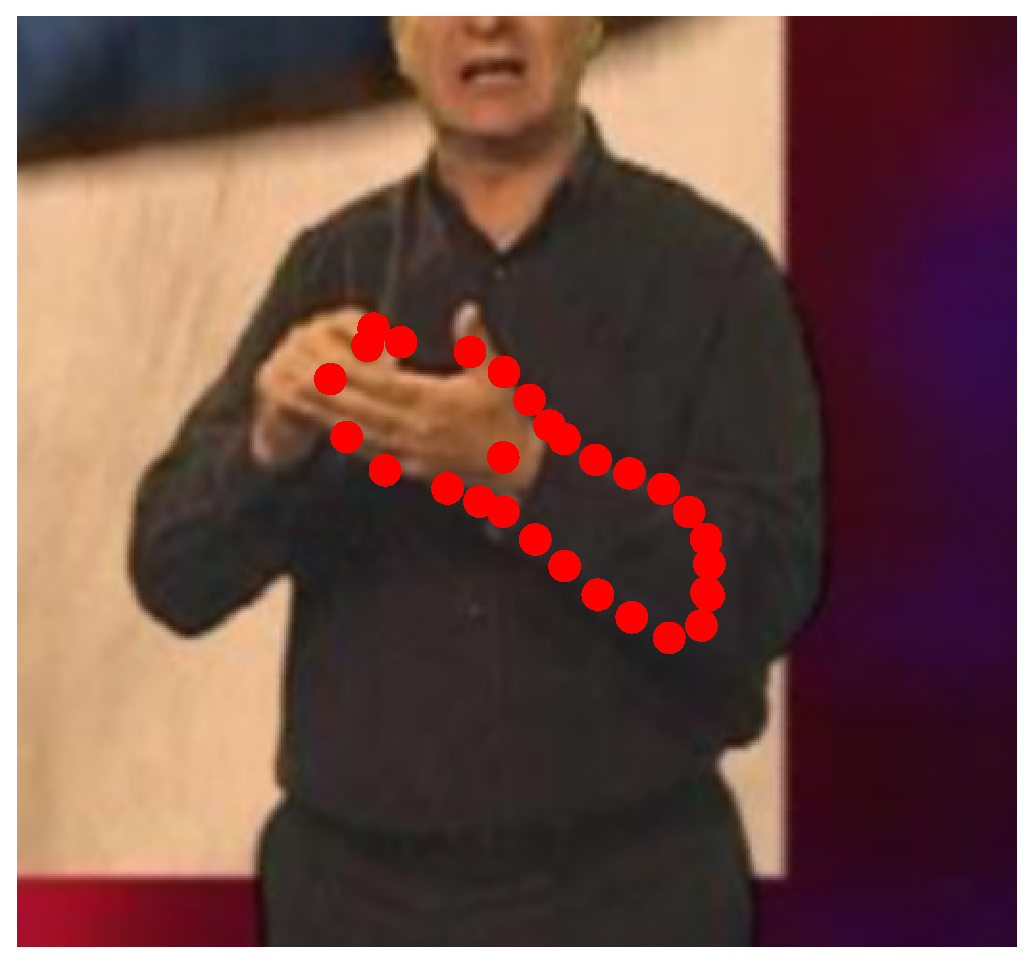
\includegraphics[height=\ofh]{Suplementory_Meterial/ExFit/0040.eps}
    \hfill
    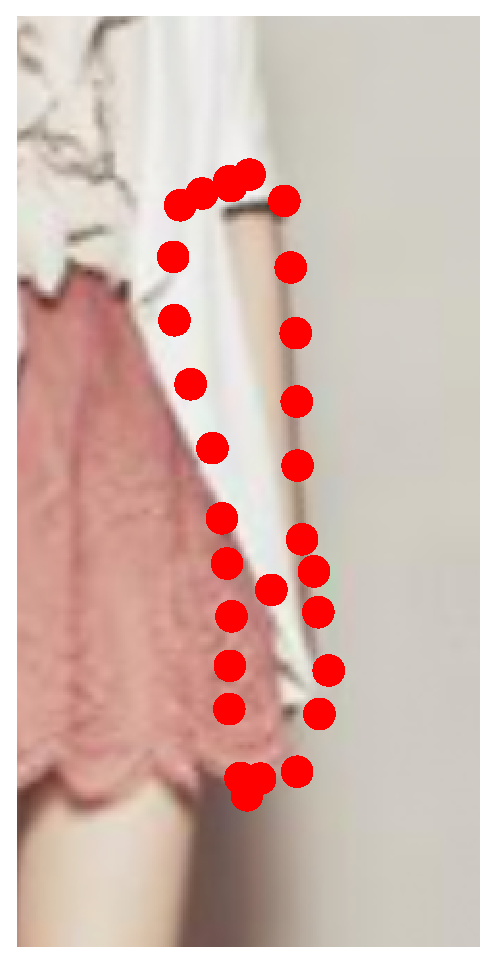
\includegraphics[height=\ofh]{Suplementory_Meterial/ExFit/0041.eps}
    \hfill
    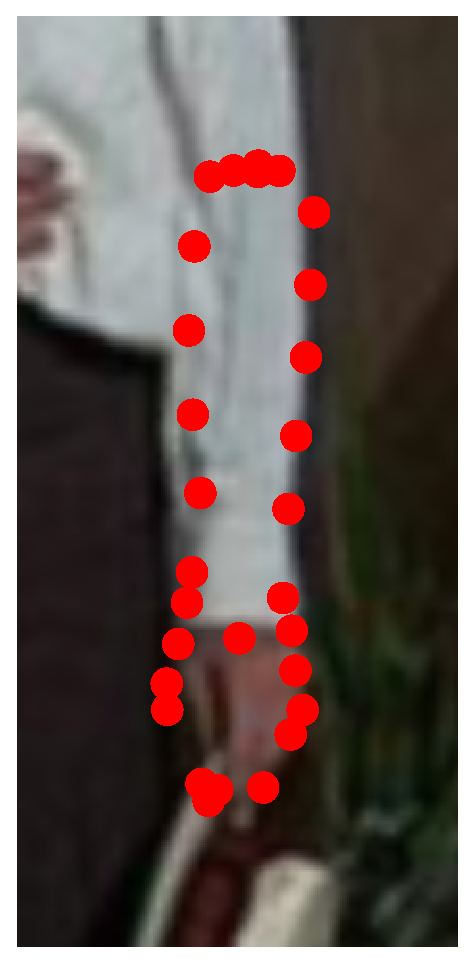
\includegraphics[height=\ofh]{Suplementory_Meterial/ExFit/0042.eps}
    \hfill
    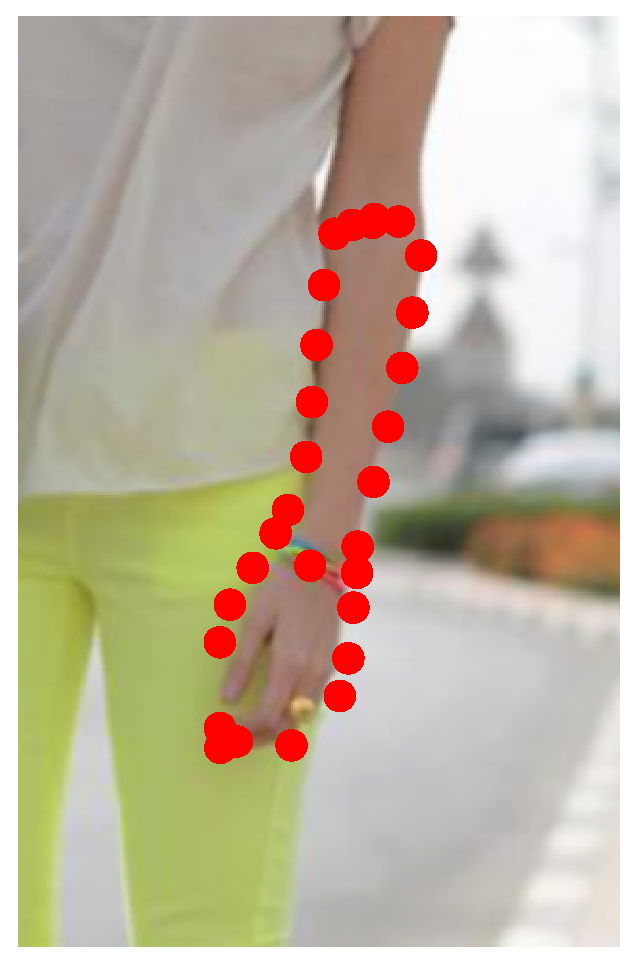
\includegraphics[height=\ofh]{Suplementory_Meterial/ExFit/0043.eps}
    \hfill
    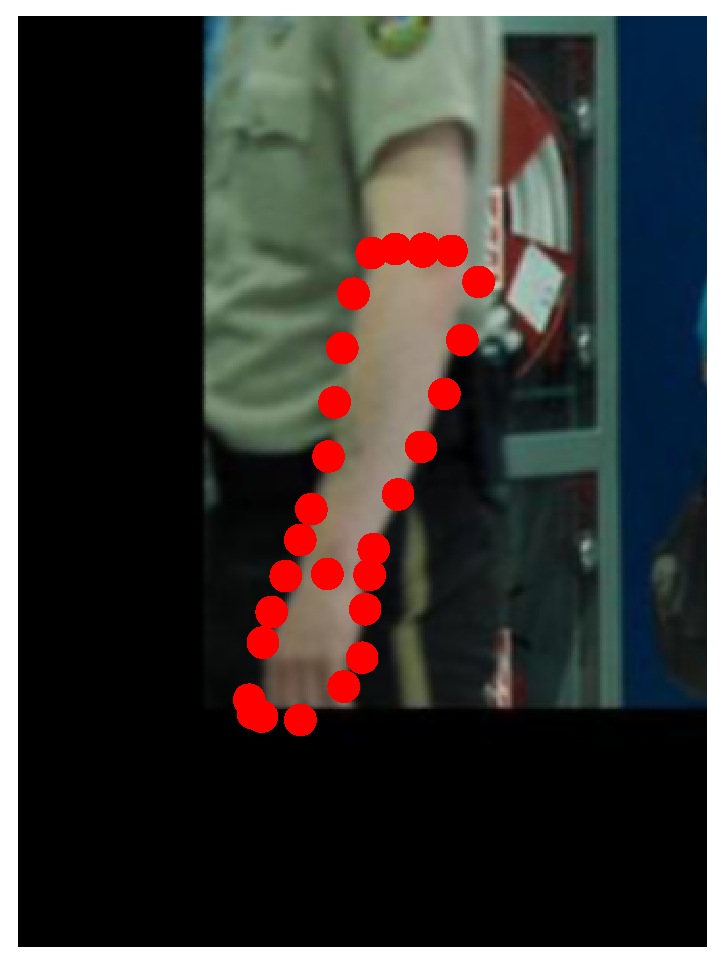
\includegraphics[height=\ofh]{Suplementory_Meterial/ExFit/0044.eps}
    \caption{Demonstration of outline fitting of patch-based AAM on arms. Images are cropped to arms only for better visualisation.}
    \label{fig:paam_fittingresults}
\end{figure*}

This section shows spares annotation of densely corespondent shapes are generated, since patch-based AMM support consistent parse annotation only in section~\ref{sec:sparsesample}. Also, shape model visualisation of build patch-based AMM are shown in section~\ref{sec:paam_sm}, as well as corresponding fitting result visualisation are shown in section~\ref{sec:paam_fittingresults}.


\subsection{Subsampling Sparse Outline from Dense Correspondent Shapes}
\label{sec:sparsesample}

\begin{figure}[!b]
\centering
\newcommand{\ofh}{0.24\columnwidth}
    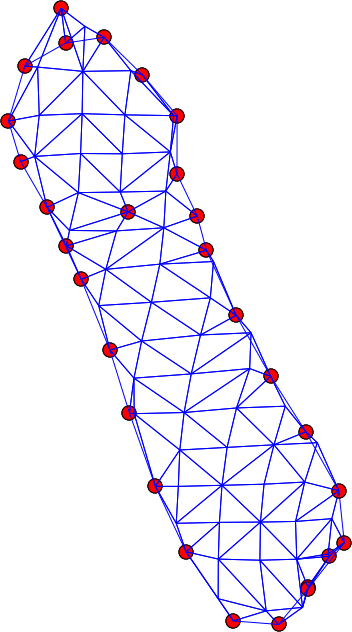
\includegraphics[height=\ofh]{Suplementory_Meterial/SparseSamples/mean.png}
    \hfill
    \includegraphics[height=\ofh]{Suplementory_Meterial/SparseSamples/mean-0.png}
    \hfill
    \includegraphics[height=\ofh]{Suplementory_Meterial/SparseSamples/mean-1.png}
    \hfill
    \includegraphics[height=\ofh]{Suplementory_Meterial/SparseSamples/mean-2.png}
    \hfill
    \includegraphics[height=\ofh]{Suplementory_Meterial/SparseSamples/mean-3.png}
    \hfill
    \includegraphics[height=\ofh]{Suplementory_Meterial/SparseSamples/mean-4.png}
\caption{Demonstration of sparse sampling from dense shapes. Left most image shows sparse sample on the reference shape while other 5 images shows projection from sampled reference shape to arbitrary shapes with dense correspondence.}
\label{fig:sparsesample}
\end{figure}

As \emph{step 4} in main paper refers, patch-based AAM are suitable for fitting objects that interior appearance having no structure, in this case e.g. arms. But patch-based AAM require consistent sparse annotation. So a sub-sampling step is needed to meet such criteria. As we built dense correspondence between shapes, we only sparsely annotate one shape so rest shapes are sub-sampled automatically since sparse samples are preserved in all shapes by dense correspondence generated with shape flow. Figure~\ref{fig:sparsesample} shows sparse annotation (red dots) on dense mean shape (grid visualisation used for visibility) and exemplar projected samples on other shapes.

\subsection{Patch-based AAM Shape Model}
\label{sec:paam_sm}

\begin{figure}[!b]
\centering
\includegraphics[width=\columnwidth]{Suplementory_Meterial/HandSMPAAM/handsmpaam}
\caption{Principal components of patch-based AAM built on arms.  The mean (left most column) as well asthe first four principal components are visualised with three times the variance of the corresponding component it used in each case.}
\label{fig:paam_sm}
\end{figure}

Figure~\ref{fig:paam_sm} shows mean shape and corresponding $\pm 3$ variation on first four principle components. As the appearance model are built with SIFT feature, the 36-channel feature give no meaningful visualisation to human so we have not shown it. From arms shape model, we observe that the variation of shape captured by the model are reasonable.

\subsection{Fitting Results}
\label{sec:paam_fittingresults}

\begin{table}[t!]
    \small
    \centering
    \begin{tabular}{|l|c|c|c||c|c|c|}
        \hline
                            & \multicolumn{3}{c||}{Wrist} & \multicolumn{3}{c|}{Elbow}\\
        \hline
        \emph{Method}       & \emph{mean} & \emph{std} & $\leq 6pt$ & \emph{mean} & \emph{std} & $\leq 6pt$\\
        \hline\hline
        Buehler             & 12.08    & 19.94        & 44.5\%       & 12.94    & 14.65        & 34.4\%\\
        Charles14           & 11.81    & 20.89        & 54.2\%       &  8.30    & 11.00        & \textbf{55.2\%}\\
        Charles13           & 13.78    & 22.39        & 43.3\%       & 13.17    & 18.74        & 46.3\%\\
        Pfister14           & 14.69    & 17.89        & 29.7\%       & 14.60    & 10.59        & 14.0\%\\
        Ramanan             & 15.59    & 19.04        & 22.6\%       & 15.53    & 10.82        & 15.8\%\\
        Pfister15           & 7.62     & 11.04        & 54.1\%       &  8.84    & 11.44        & 54.9\%\\
        \hline\hline
        Ours                & \textbf{6.71}& \textbf{10.90}   & \textbf{63.1\%}       & \textbf{8.20}     &  \textbf{10.54}        & 52.1\%\\
        \hline
    \end{tabular}
    \caption{Fitting statistics on BBC Pose database for experiment 4.2 in main paper.}
    \label{tab:hand_benchmark}
\end{table}
    
Figure~\ref{fig:paam_fittingresults} demonstrates more fitting results produced by fitting patch-base AAM on arms datasets including MPII \cite{andriluka14cvpr}, Fashion Pose \cite{dantone2013human}, FLIC \cite{sapp2013modec} and BBC Poses \cite{pfister2015flowing}. All fittings are initialised using same method as mention in experiment 4.2 in main paper.

In addition table~\ref{tab:hand_benchmark} presents statistics results that refers to experiment 4.2 in main paper for additional information. Column $\leq 6pt$ reports the percentage of fittings that having errors, point-to-point distance on normalised images, less than 6 pixels (same measurement used in \cite{pfister2015flowing}). This shows we have notable improvement on estimating wrists and comparable results on estimating elbow.

{\small
\bibliographystyle{ieee}
\bibliography{bib}
}


\end{document}









% \subsection{Appearance Reconstruction}
% \label{sec:reconstruct}

% \begin{figure}[!b]
%     \centering
%     %\vspace*{-0.2in}
%     \includegraphics[width=0.5\textwidth]{Suplementory_Meterial/Fig_Draw/draw}
%     \caption{Synthesizing face images from caricature sketches. First column: caricature sketches. Second column: arbitrary chosen face images. Third and last column: sketch-based warping of images based on AAMs (third column) and dAAMs (last column).}
%     \label{fig:draw}
% \end{figure}

% In this qualitative experiment, we show how the proposed pipeline can be used to generate novel modified instances of an object, e.g. caricatures. To be specific, firstly we manually craft a set of hand-drawn cartoon-like shape sketches. We then apply shape flow to align them with the reference frame. In this way, we establish dense correspondences of landmarks. Afterwards, we perform shape reconstruction using both AAMs and dAAMs. Finally, we warp the appearance from arbitrarily chosen faces on the reconstructed shape using either piecewise affine warp (in the case of AAMs) or shape flow (in the case of dAAMs). The corresponding results are shown in figure \ref{fig:draw}. We see that AAMs introduce more severe artifacts, especially on the areas of mouth and eyes, where nuanced information is missing or models are overly deformed. In contrast, dAAMs yield a significantly more plausible result.



% \section{Segmentation using Dense AAM}
% \label{sec:segmentation}

% In this section, we present experiments of utilising our dense AAM for object segmentation. Two object classes, bottles and human bodies, are considered. For human bodies, we use images along with ground truth segmentation from Space-Time Actions dataset \footnote{\label{sta} \url{http://www.wisdom.weizmann.ac.il/~vision/SpaceTimeActions.html}}, which includes sequences with several human actions. We use ``jumping'' and ``sliding'' actions. As far as bottles are concerned, we use 500 high-resolution images that we collected and annotated using a newly-defined 50 point annotation scheme, as well as the curve annotations proposed in this paper. We randomly split these images into two disjoint sets of training (400) and testing (100) images. Bottle models were built using 400 training images while body models are built in terms of human actions (e.g. jumping), each having approximately 200 training images and 50 test images.

% \begin{figure}[!t]
%     \centering
%     \begin{subfigure}[b]{0.15\textwidth}
%             \includegraphics[height=\textwidth]{Suplementory_Meterial/Segmentation_Measure/ear}
%         %\caption{Ear Initial Bounding Box}
%     \end{subfigure}
%     \begin{subfigure}[b]{0.15\textwidth}
%             \includegraphics[height=\textwidth]{Suplementory_Meterial/Segmentation_Measure/bottle}
%         %\caption{Bottle Initial Bounding Box}
%     \end{subfigure}
%     \begin{subfigure}[b]{0.15\textwidth}
%             \includegraphics[height=\textwidth]{Suplementory_Meterial/Segmentation_Measure/body}
%         %\caption{Body Initial Bounding Box}
%     \end{subfigure}
%     \caption{Examples of fitting initialisations used for the segmentation experiment. These are created by random perturbation of the ground-truth bounding box.}
%     \label{fig:seg_init}
% \end{figure}

% Fitting dAAMs on test images yields dense landmarks that can be used to perform segmentation. In a real-world scenario, a simple object detector would be required to be applied prior to our pipeline to initialise the fitting. However, as a simple evaluation, we initialise the fitting by randomly perturbing the ground-truth bounding box with certain variance to simulate an object detector with implicit detection, see e.g.~Figure \ref{fig:seg_init}. Table  \ref{tab:seg_result} reports the segmentation precision, in case of fitting bottles and human bodies by adopting the proposed dAAMs pipeline.

% \begin{table}[!h]
% \small
% \centering
% \begin{tabular}{|l|c|c|c|}
% \hline
% \emph{Object}   & \emph{mean} & \emph{std} & \emph{median}\\
% \hline\hline
% Bottles         & 0.8125      & 0.1460     & 0.8414\\
% Action - Jump   & 0.6102      & 0.0198     & 0.6099\\
% Action - Slide  & 0.6444      & 0.0500     & 0.6501\\
% \hline
% \end{tabular}
% \caption{Segmentation precision, in case of fitting bottles and human bodies by adopting the proposed dAAMs pipeline. The mean, standard deviation and median of the precision error are provided.}
% \label{tab:seg_result}
% \end{table}